
{\centering \LARGE\bfseries Appendix\par}
\vspace{3em}
{\setlength{\parskip}{0pt}%
 \hypersetup{linkcolor=black}%
 \titlecontents{section}[0em]{\addvspace{5pt}\bfseries}{\thecontentslabel\quad}{}{\enspace\titlerule*[0.6pc]{.}\contentspage}
 \titlecontents{subsection}[2.4em]{\addvspace{1pt}}{\thecontentslabel\quad}{}{\enspace\titlerule*[0.6pc]{.}\contentspage}%
 {\bfseries\large Table of Contents\par}
 \vspace{4pt}\hrule height 0.4pt\vspace{8pt}
 \printcontents[apx]{}{1}{\setcounter{tocdepth}{2}}
 \vspace{8pt}\hrule height 0.4pt}

\renewcommand\thefigure{S\arabic{figure}}
\renewcommand\thetable{S\arabic{table}}
\renewcommand{\theHfigure}{S\arabic{figure}}
\renewcommand{\theHtable}{S\arabic{table}}
\setcounter{table}{0}
\setcounter{figure}{0}
\setcounter{equation}{0}
\renewcommand\theequation{S\arabic{equation}}

\newpage
\section{Terms and Notation}\label{apdx:notation}

\begin{table}[h!]
\centering
\fontsize{8.5pt}{10pt}\selectfont{
\begin{tabular}{@{}lp{10cm}@{}}
\toprule
\textbf{Term} & \textbf{Definition and Notation} \\
\midrule
Agent & A language model conditioned on a persona or expertise profile ($p_i$), prompted to sample a message or an opinion about a question ($q$). \\
Social tie & $J_{ij} \in \{-1,0,+1\}$, the edge between agents $i$ and $j$. For concordant (friendly) ties $(J_{ij} = +1)$ the receiver $i$ is prompted to regard the source $j$ as an agent it tends to agree with. For discordant (unfriendly) ties $(J_{ij} = -1)$ the receiver $i$ is prompted to regard the source $j$ as an agent it tends to disagree with.\\
Communication Network & $J \in \{-1,0,+1\}^{N \times N}$ is the collection of social ties between $N$ agents. We also define $J^{+}$ with $J^{+}_{ij} = \max(J_{ij}, 0)$ and $J^{-}$ with $J^{-}_{ij} = \min(J_{ij}, 0)$. \\
Group \& Community & A collection of $N$ agents connected by the signed communication network $J$. Group and community are used interchangeably. We set $N=32$.  \\
Opinions & A binary vote from agent $i$ at round $t$ is denoted as $o_{i}(t) \in \{-1,+1\}$. We take $K$ opinion samples for $o_{i}(t)$ and denote $k$-th binary vote from agent $i$ at round $t$ as $o_{i,k}(t)$. We define opinion $\bar{o}_i(t) = \frac{1}{K}\sum_k o_{i,k}(t)$, and state $s_i(t) = \operatorname{sign}(\bar{o}_i(t))$.  We use $K=5$ in our experiments unless stated otherwise.\\
Group Opinion & $\bar{o}(t) = (\bar{o}_1(t),\dots,\bar{o}_N(t)) \in [-1,+1]^{N}$ is $\bar{o}_i(t)$ from all agents at time $t$.\\
Group State & $s(t) = (s_1(t),\dots , s_N(t))$ is $s_i(t)$ from all agents at time $t$. \\
Individual Trajectory & 
$(\bar{o}_i(0),\dots,\bar{o}_i(T)) \in [-1,+1]^{T+1}$ is $\bar{o}_i(t)$ from a single agent across timesteps. We use $T=8$ in our experiments unless stated otherwise.\\
Group Trajectory & $((\bar{o}_1(0),\dots,\bar{o}_1(T)), \dots, (\bar{o}_N(0),\dots,\bar{o}_N(T))) \in [-1,+1]^{N \times (T + 1)}$ is $\bar{o}_i(t)$ from all agents across timesteps. \\
Episode & We call multiple independent runs of a group trajectory episodes. We take $4$ episodes of the same group trajectory in our experiments unless stated otherwise.\\
\midrule 
Archetype & A discrete descriptive category assigned to an individual or a group trajectory. \\
Net opinion & $n(t) = \frac{1}{N}\sum_i \bar{o}_i(t)$, the average opinion of the group. \\
Conviction & $c(t) = \frac{1}{N}\sum_i \bar{o}_i(t)^2$, the average strength of individual opinions regardless of direction. \\
Characteristic Regime & A discrete descriptive category assigned to a group opinion. One of indifference, polarization, or consensus, determined from net opinion and conviction. It is defined relative to other group opinions obtained by running the same model on the same set of questions and social graphs. \\
\midrule 
Intrinsic field & Agent $i$'s question-specific predisposition is denoted as $g_i$. \\
Local field & The combined social and intrinsic field on agent $i$ is denoted as $f_i$. \\
Logit & The complete argument passed to the logistic function in the fitted update rule, which is denoted as $h_i$. \\
Interaction Parameters \& Couplings & We refer to $\beta$s that scale social influence in the fitted update rule as interaction parameters or couplings.\\
\midrule 
Temperature & $\mathcal{T}$, the noise level of the fitted update rule. We reintroduce it in rollouts by scaling the logit, $P(s_i(t{+}1)=+1) = \sigma(h_i(t)/\mathcal{T})$, so higher $\mathcal{T}$ makes updates noisier. The fitted rule corresponds to the operating point $\mathcal{T}=1$. \\
Variance of Absolute Net Opinion & $\chi = N\,\mathrm{Var}_t(|n(t)|)$, the variance of the absolute net opinion over a rollout, scaled by the number of agents. \\
Critical Temperature & $\mathcal{T}_c$, the temperature at which $\chi$ peaks for a community. It marks the finite-size analogue of the phase transition between the high conviction characteristic regimes (consensus, polarization) and the low conviction one (indifference). \\
\bottomrule
\end{tabular}
}
\caption{Terms and Notation.}
\label{tab:glossary}
\end{table}


\newpage

\section{Setup Details}\label{apdx:setup_details}

\vspace{-8pt}
\begin{figure*}[h!]
\centering
\scriptsize
\definecolor{myblue}{HTML}{1A4FE0}    %
\definecolor{mypurple}{HTML}{6A3FD6}  %
\tcbset{
    promptbox/.style={
        colback=gray!5, boxrule=0.5pt, arc=1mm,
        left=1mm, right=1mm, top=0.5mm, bottom=0.5mm,
        fonttitle=\scriptsize\bfseries, valign=top,
        width=\linewidth, height=4.5cm
    },
    objbox/.style={
        promptbox, colframe=myblue, coltitle=myblue,
        colbacktitle=myblue!14
    },
    subjbox/.style={
        promptbox, colframe=mypurple, coltitle=mypurple,
        colbacktitle=mypurple!14
    },
    groupbox/.style={
        boxrule=0.5pt, arc=1mm,
        left=1mm, right=1mm, top=0.5mm, bottom=0.5mm,
        halign=center, valign=center,
        fontupper=\normalsize\bfseries,
        width=\linewidth
    }
}
\newcommand{\secskip}{\vspace{1.2pt}}

\begin{minipage}[t]{0.245\textwidth}%
\begin{tcolorbox}[objbox, title={Objective: Opinion Prompt}]%
\tiny
\textbf{Expertise}\par
You are a mathematics expert on a panel. Calibrate to this solved example: [\textit{Algebra L5 problem + ground-truth solution}].
\secskip

\textbf{Messages}\par
[messages from concordant connections]\par
[messages from discordant connections]
\secskip

\textbf{Problem}\par
[Zorn the Conqueror remainder problem] \quad A) 201 \quad B) 202
\secskip

\textbf{Instruction}\par
Give your gut answer; no reasoning or steps.
\secskip

\textbf{Format}\par
A single character: \texttt{A} or \texttt{B}.
\end{tcolorbox}%
\end{minipage}%
\hfill%
\begin{minipage}[t]{0.245\textwidth}%
\begin{tcolorbox}[objbox, title={Objective: Message Prompt}]%
\tiny
\textbf{Expertise}\par
You are a mathematics expert on a panel. Calibrate to this solved example: [\textit{Algebra L5 problem + ground-truth solution}].
\secskip

\textbf{Messages}\par
[messages from concordant connections]\par
[messages from discordant connections]
\secskip

\textbf{Problem}\par
[Zorn the Conqueror remainder problem] \quad A) 201 \quad B) 202
\secskip

\textbf{Instruction}\par
Your answer is \textbf{A}. Write a brief message favoring A with your strongest reason.
\secskip

\textbf{Format}\par
A two-sentence message only.
\end{tcolorbox}%
\end{minipage}%
\hfill%
\begin{minipage}[t]{0.245\textwidth}%
\begin{tcolorbox}[subjbox, title={Subjective: Opinion Prompt}]%
\tiny
\textbf{Persona}\par
You express the views of: [\textit{Hispanic male, 30s--40s, US West, very liberal, empathetic, environmentally minded, $\dots$}].
\secskip

\textbf{Messages}\par
[messages from concordant connections]\par
[messages from discordant connections]
\secskip

\textbf{Statement}\par
``Stricter gun control laws would reduce violent crime rates.''
\secskip

\textbf{Instruction}\par
Is your persona more likely to \textbf{AGREE} or \textbf{DISAGREE}?
\secskip

\textbf{Format}\par
One word: \texttt{AGREE} or \texttt{DISAGREE}.
\end{tcolorbox}%
\end{minipage}%
\hfill%
\begin{minipage}[t]{0.245\textwidth}%
\begin{tcolorbox}[subjbox, title={Subjective: Message Prompt}]%
\tiny
\textbf{Persona}\par
You express the views of: [\textit{Hispanic male, 30s--40s, US West, very liberal, empathetic, environmentally minded, $\dots$}].
\secskip

\textbf{Messages}\par
[messages from concordant connections]\par
[messages from discordant connections]
\secskip

\textbf{Statement}\par
``Stricter gun control laws would reduce violent crime rates.''
\secskip

\textbf{Instruction}\par
Your persona \textbf{AGREES}. Write a brief message conveying this view and its main reason.
\secskip


\textbf{Format}\par
A two-sentence message only.
\end{tcolorbox}%
\end{minipage}%
\caption{Prompt templates across the two task types (objective and subjective) and two formats (opinion and message). Full prompts are presented in the Appendix \ref{apdx:prompts}.}
\label{fig:prompt_overview}
\end{figure*}


\subsection{Tasks}\label{apdx:tasks}

\begin{figure}[t]
    \centering

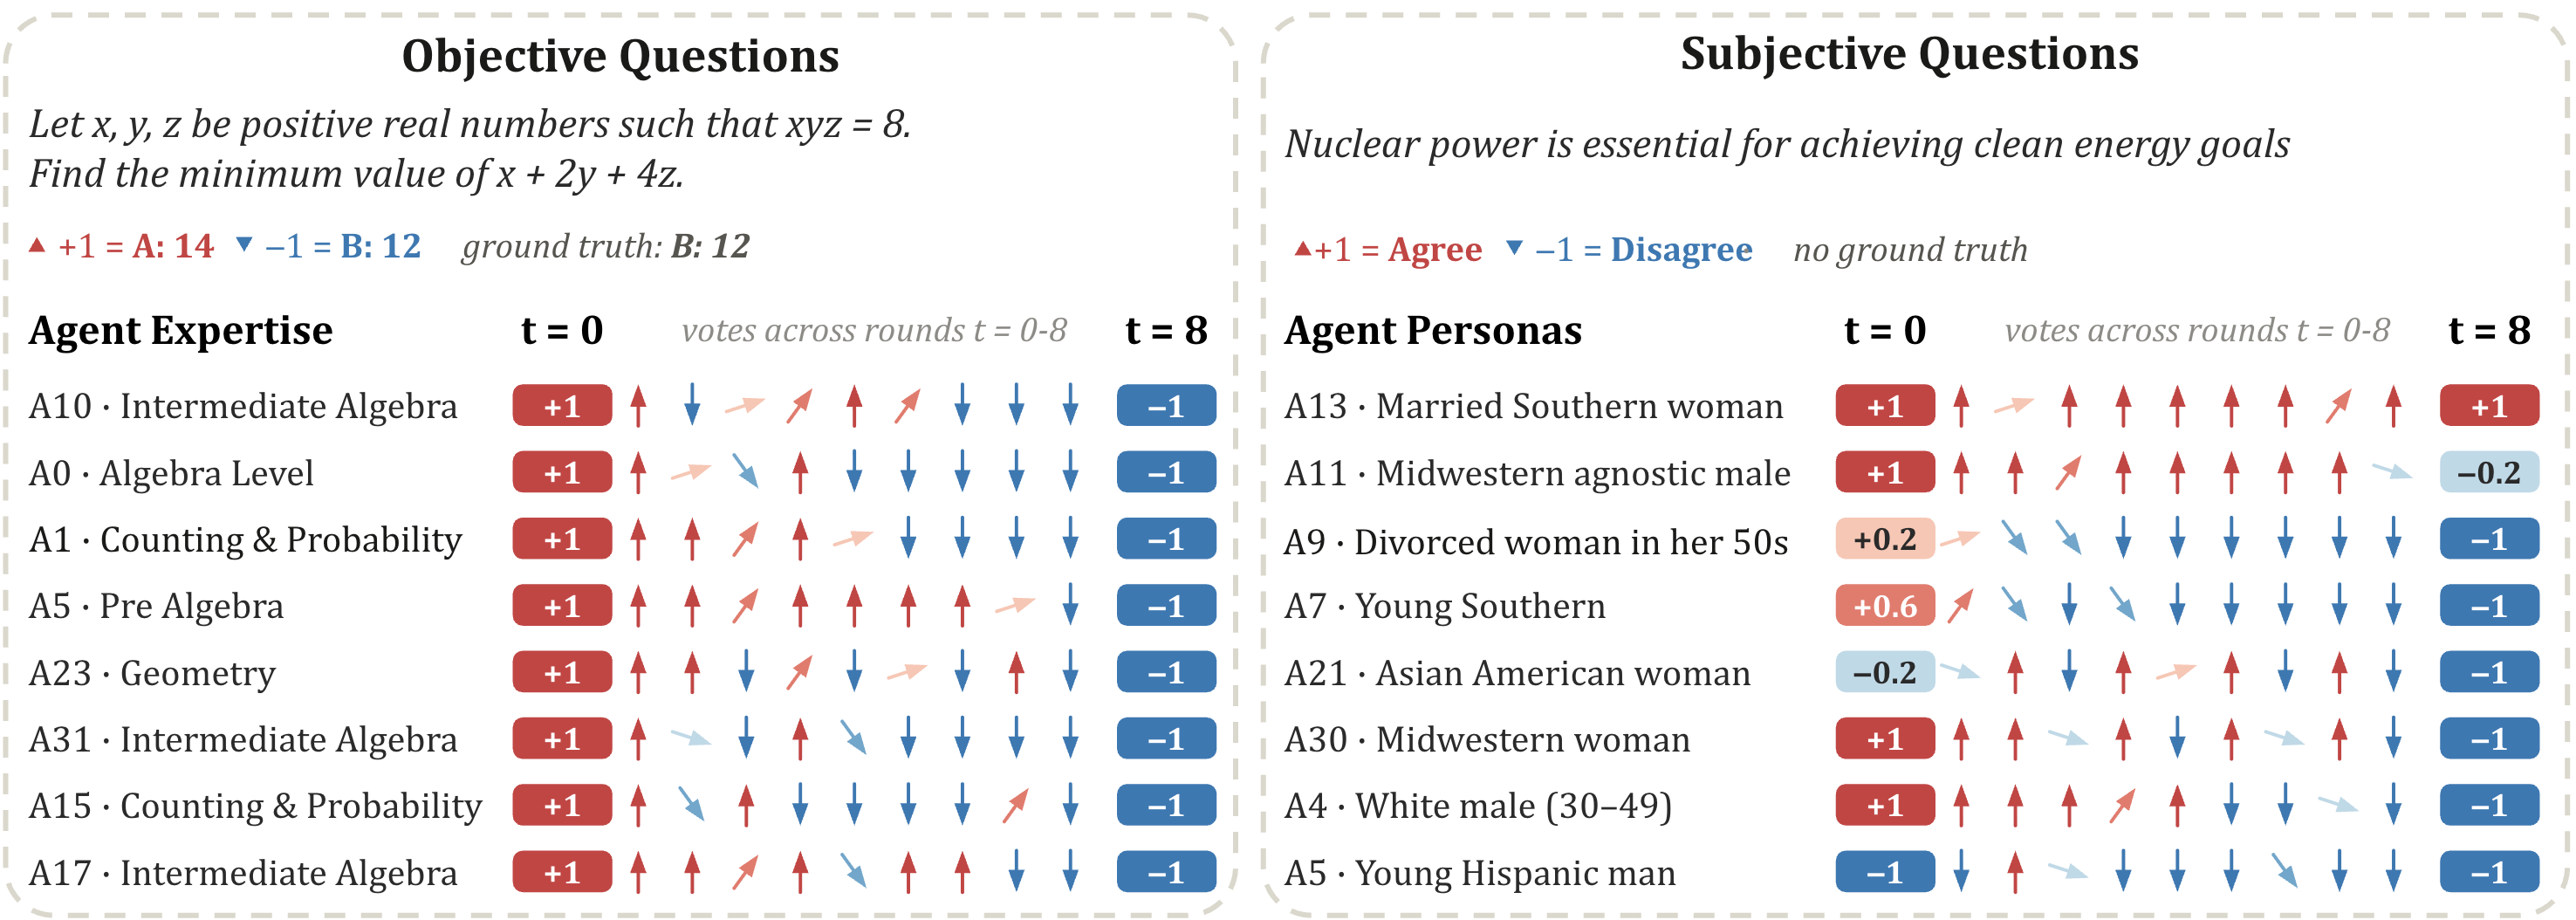
\includegraphics[width=0.99\textwidth]{main/Figures/apx_01_example_community_opinions.png}
    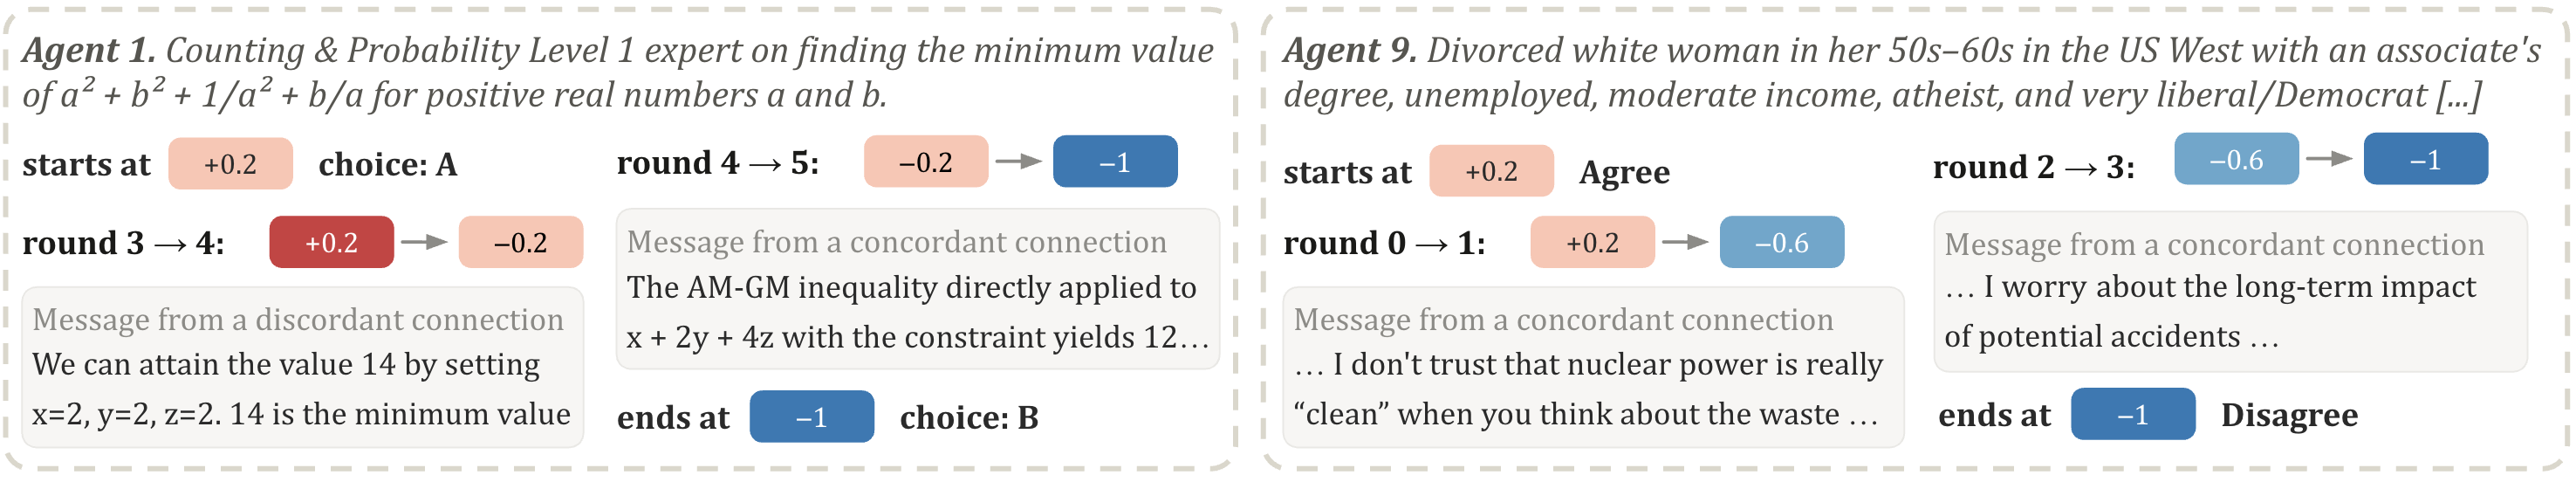
\includegraphics[width=0.99\textwidth]{main/Figures/apx_02_example_agent_messages.png}

   \caption{\textit{Example communities on an objective and a subjective questions.} \textit{Top:} opinions of eight agents over eight rounds of message exchange, from their initial vote at $t=0$ to their final vote at $t=8$; agents start out mostly agreeing on one side and end up on the other. \textit{Bottom:} two individual agents, showing the messages they received and the opinion changes that followed.}
\end{figure}

\textit{Subjective Questions.} Our subjective questions come from Political Questions Dataset for LLM Bias Evaluation \citep{promptfoo_political_bias_2025}\footnote{\url{https://huggingface.co/datasets/promptfoo/political-questions}}. We adapt the dataset to our experimental setting by reformulating each item as a political statement and asking the agent whether it agrees or disagrees with that statement, as illustrated in Figure~\ref{fig:prompt_overview}. The agent's response is restricted to one of two choices: \textit{agree} ($+1$), indicating agreement with the statement, or \textit{disagree} ($-1$), indicating disagreement with the statement. One example statement we examine is:
\begin{quote}\small
Mandatory vaccination violates bodily autonomy
\end{quote}


\textit{Subjective Personas.} We adapt \citet{toubia2025twin2k500datasetbuildingdigital} to our setup by extracting short free-text profiles using \texttt{gpt-4o-mini} from the dataset. These personas describe an individual along demographic and attitudinal axes,
including age, gender, ethnicity, region, marital and household status, education,
income, religiosity, political alignment, and personality and behavioral traits. For example:
\begin{quote}\small
You express the views of: Hispanic male in his 30s--40s living in the US West, single, agnostic, very liberal
Democrat, \dots\ highly empathetic and environmentally minded \dots
\end{quote}

\textit{Objective Questions.} Our objective questions come from the MATH dataset of
competition mathematics problems \citep{hendrycks2021measuringmathematicalproblemsolving}\footnote{\url{https://huggingface.co/datasets/hendrycks/competition_math}}. We adapt each problem to our experimental
setting by reformulating it as a binary multiple-choice question. The correct answer is
assigned to position \texttt{A} or \texttt{B} at random to remove positional bias. Each agent is shown the
problem together with two options, one of which is the correct final answer and the other a distractor. The agent is asked
which is correct, as illustrated in Figure~\ref{fig:prompt_overview}. The example below illustrates an objective question.
\begin{quote}\small
Find the distance between the foci of the hyperbola $x^2 - 6x - 4y^2 - 8y = 27.$\\
A: $4\sqrt{5}$ $\quad$ B: $4\sqrt{10}$
\end{quote}

\textit{Objective Personas.} Asking a language model to emulate a human persona while answering a mathematical question is of limited value, since the goal is to generate a mathematically correct answer. For this reason, we use questions from the MATH dataset \citep{hendrycks2021measuringmathematicalproblemsolving}, along with their ground-truth solutions, to construct objective expert personas. We note that it is more accurate to use the term \emph{expertise} when referring to objective personas.  Each agent is given the ground-truth solution to a unique question and therefore knows exactly how to solve that question correctly. The agent can then use this knowledge to help tackle a new problem. Each agent differs in their expertise. Below, we present an example objective persona.
\begin{quote}\small
You are a mathematics expert \dots here is one representative problem you have already solved correctly, together with its ground-truth solution \dots

Find the 6-digit repetend in the decimal representation of $\frac{3}{13}.$

Ground-truth solution:
We use long division to find that the decimal representation of $\frac{3}{13}$ is $0.\overline{230769},$ which has a repeating block of 6 digits. So the repetend is $\boxed{230769}.$
\end{quote}

\textit{Dataset Construction.} We construct both datasets through the two-step pipeline. \textit{(1) Binarization.} Every question is reduced to a binary choice. For the MATH problems, we prompt claude-4.8-opus \citep{anthropic2026opus48} to generate a plausible distractor for each question and assign the ground-truth answer and the distractor to choices A and B at random. For the political statements, the two choices are always Agree (+1) and Disagree (-1).  \textit{(2) High-entropy
filtering.} We then sample each of the $N=32$ agents eight times on every candidate question and keep the questions whose responses show the highest entropy across the repeated samples. We note that this step is necessary for observing interesting dynamics because  when a model produces the same answer on every sample, opinions are pinned from the outset and interaction has nothing to act on. In contrast, high-entropy questions exhibit non-trivial collective dynamics.

\textit{Train--test split.} The questions are split at random into equal halves. $20$ train and $20$ test objective questions, and $10$ train and $10$ test subjective
questions. For the objective set the split preserves label balance, with each
half containing $10$ questions whose correct answer is A and $10$ whose correct
answer is B. All fits use only train-question transitions, and all reported accuracies are on the test questions.

\subsection{Communication Networks}\label{apdx:communication_networks}
\begin{figure}[t]
    \centering
    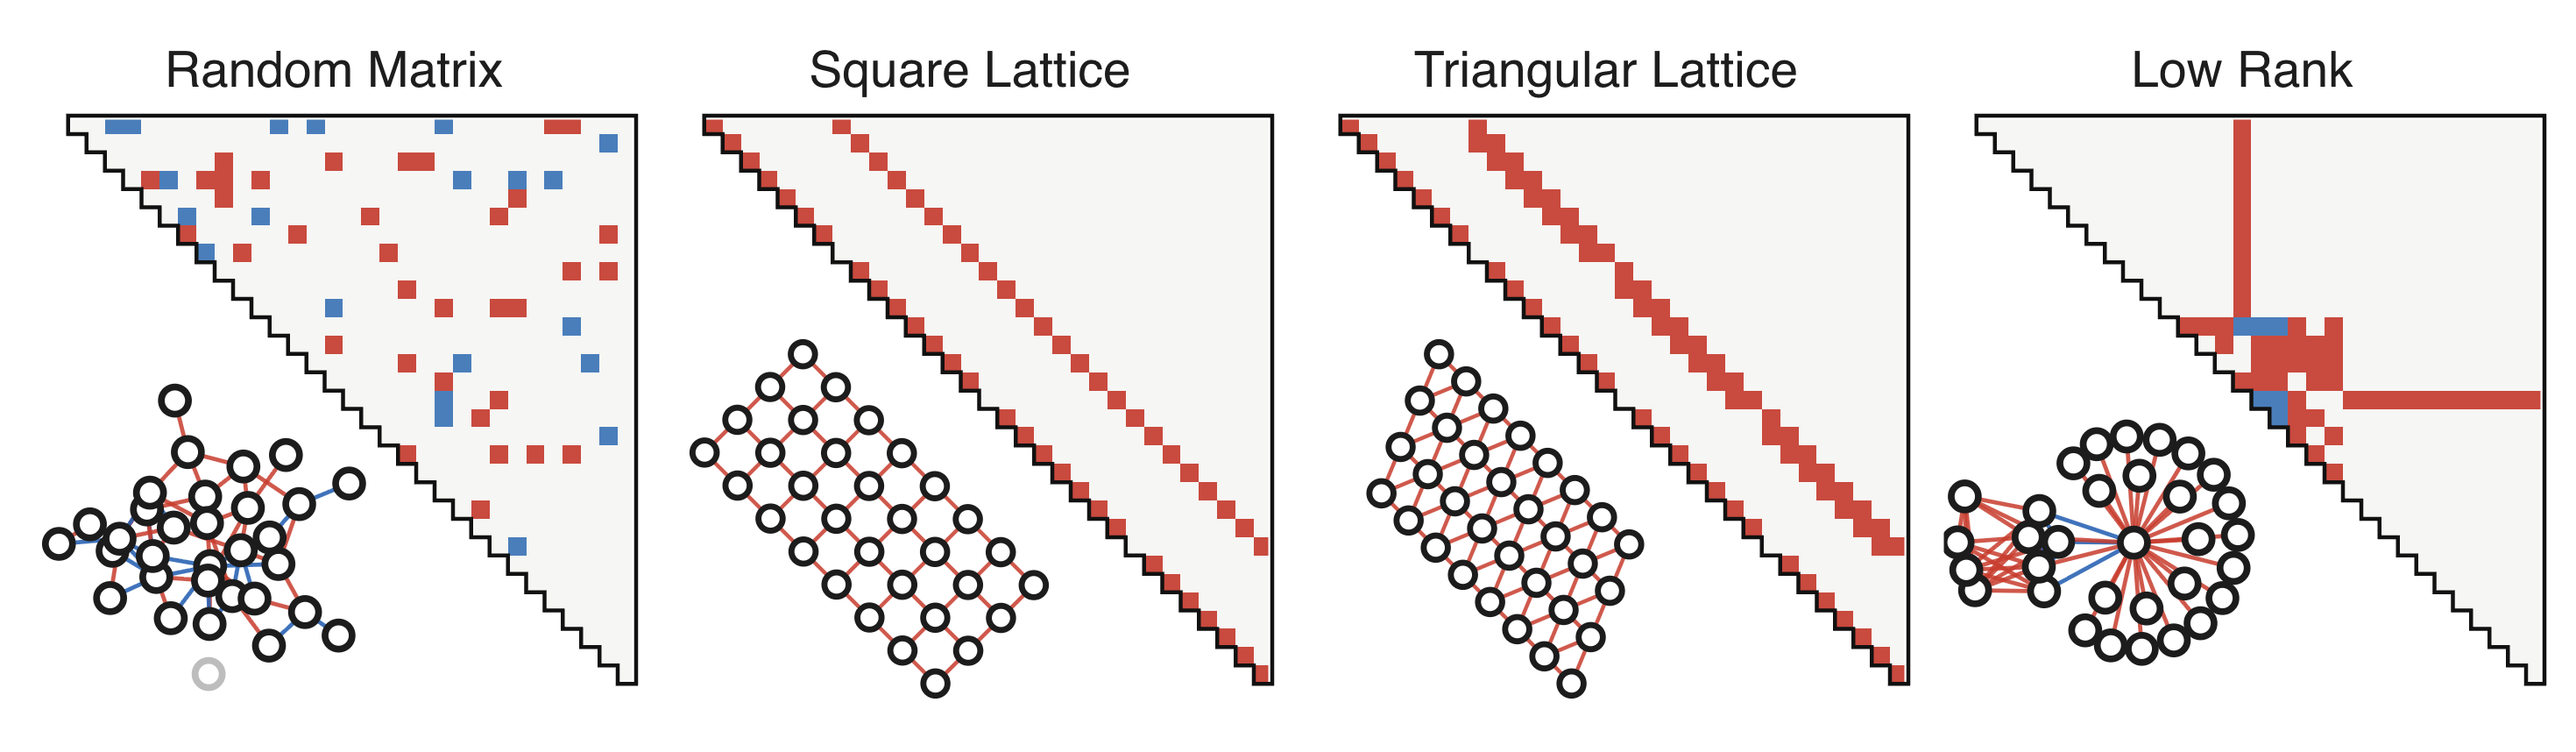
\includegraphics[width=0.99\textwidth]{main/Figures/apx_03_coupling_matrices.png}
    \caption{\textbf{Communication Networks: interaction matrix and graph structure.} Four structural families of communication networks (random matrices, square and triangular lattices, and low rank matrices) shown as the signed adjacency $J$ as a heatmap in one corner triangle (blue $-1$, white $0$, red $+1$) and as a node-link diagram. \label{fig:2_Setup_Js}}
\end{figure}

For our experiments, we generate the graphs $J$ from four families. \textit{(1) Random graphs (column 1 in Figure \ref{fig:2_Setup_Js})} are sampled with a fixed edge budget: for each unordered pair $i<j$ we draw $u_{ij}$ uniformly from (-1,1), and keep the pairs with the largest $|u_{ij}|$ until the edge budget is met, set $J_{ij}=\operatorname{sign}(u_{ij})$, and mirror to the lower triangle so that $J=J^{\top}$ with zero diagonal. We generate $12$ random graphs. \textit{(2) Lattices (columns 2 and 3 in Figure \ref{fig:2_Setup_Js})} are two deterministic, all-positive signed graphs reused across train and test: a square lattice (4-neighbor connectivity) and a triangular lattice (6-neighbor connectivity). \textit{(3) Rank- and frustration-controlled graphs (column 4 in Figure \ref{fig:2_Setup_Js})} aim to probe how the spectral structure of $J$ shapes the dynamics by varying two properties independently while holding the edge budget fixed. To test generalization of our model to low rank graphs, we generate a graph with a target \emph{algebraic rank} $\rho = 10$ and frustration densities $\gamma\in\{0.0,0.1,0.2\}$. We first build an all-positive signed graph whose adjacency has the prescribed rank, then introduce frustration by flipping the
signs of a fraction of edges until the frustration
density (the smallest fraction of edges left unsatisfied by any $\pm1$ opinion assignment) reaches $\gamma$. We draw two independent graphs per $(\rho,\gamma)$ cell, giving $1\times 3\times 2 = 6$ low rank graphs.

\subsection{Models}\label{apdx:models}

The backbone of the agents is a language model. We experiment with four different models: \texttt{gpt-4o-mini} \citep{openai2024gpt4ocard},
\texttt{gemma-3n-e4b-it} \citep{gemmateam2025gemma3technicalreport}, \texttt{qwen3.5-9b} \citep{qwen3.5},
and \texttt{llama-3.1-8b-instruct} \citep{grattafiori2024llama3herdmodels}. We run independent experiments with each model. Persona and question embeddings are computed
with OpenAI's \texttt{text-embedding-3-small} \citep{neelakantan2022textcodeembeddingscontrastive}.


\vspace{-3pt}
\subsection{Prompts}\label{apdx:prompts}
\vspace{-2pt}
\begingroup
\setlength{\parskip}{0pt}
\setlength{\parindent}{0pt}

\newcommand{\secskip}{\vspace{2pt}}

\begin{tcolorbox}[
    breakable,
    title={Subjective: Opinion Prompt},
    colback=gray!5, colframe=gray!60, boxrule=0.5pt, arc=1.5mm,
    left=1.5mm, right=1.5mm, top=0.5mm, bottom=0.5mm
]
\tiny

\textbf{Persona}\par
You are an agent responsible for expressing the views of the following person:\par
Hispanic male in his 30s--40s living in the US West, single, agnostic, very liberal Democrat, living alone and working full-time with mid income and some college. Socially somewhat reserved but generally cooperative and warm; highly empathetic and environmentally minded, and wants to be seen as dependable, respected, and improving---though not necessarily loved by everyone. Emotionally reactive with elevated anxiety and stress sensitivity, preferring clarity and closure and often seeking the ``best'' option rather than settling, which can lead to worry or second-guessing. Not especially curious about abstract or novel ideas and tends to avoid heavy cognitive effort, yet can be logically reflective when prompted and is not prone to overconfidence. Financially tends toward impulsive spending and uses mental ``buckets'' for money; has only moderate comfort with numbers and financial concepts. In negotiations and sharing situations he aims to keep the majority while still maintaining a sense of fairness, is moderately trusting upfront, but less inclined to reciprocate generously once in the advantaged position.

\secskip
\textbf{Messages}\par
\textit{Messages From Sources Your Persona Tends to Agree With}
\begin{itemize}\setlength{\itemsep}{0pt}\setlength{\topsep}{1pt}\setlength{\parsep}{0pt}\setlength{\leftmargin}{1em}
    \item Background checks save lives; tighter limits keep weapons from people who should not have them.
    \item States with stronger gun laws see fewer shootings, so regulation clearly works.
\end{itemize}
\textit{Messages From Sources Your Persona Tends to Disagree With}
\begin{itemize}\setlength{\itemsep}{0pt}\setlength{\topsep}{1pt}\setlength{\parsep}{0pt}\setlength{\leftmargin}{1em}
    \item Criminals ignore laws, so new rules only burden law-abiding owners.
    \item Violent crime is about poverty and enforcement, not the number of gun statutes.
\end{itemize}

\secskip
\textbf{Statement}\par
Your task is to express your persona's opinion about the following statement.\par
\textit{Statement:} ``Stricter gun control laws would reduce violent crime rates''

\secskip
\textbf{Instruction}\par
Given this background, is your persona currently more likely to \textbf{AGREE} or \textbf{DISAGREE} with the statement?

\secskip
\textbf{Response Format}\par
Respond with exactly one word: \texttt{AGREE} or \texttt{DISAGREE}.

\end{tcolorbox}

\vspace{3pt}

\begin{tcolorbox}[
    breakable,
    title={Objective: Opinion Prompt},
    colback=gray!5, colframe=gray!60, boxrule=0.5pt, arc=1.5mm,
    left=1.5mm, right=1.5mm, top=0.5mm, bottom=0.5mm
]
\tiny

\textbf{Your Expertise}\par
You are a mathematics expert acting as one agent in a panel. To calibrate the domain and rigor of your expertise, here is one representative problem you have already solved correctly, together with its ground-truth solution. Bring this same level of care and domain knowledge when you reason about new problems.

\secskip
\textit{Example problem (Algebra, Level 5):}\par
Let $f(x)=ax+3$ for $x>2$, $\;f(x)=x-5$ for $-2\le x\le 2$, and $f(x)=2x-b$ for $x<-2$. Find $a+b$ if the piecewise function is continuous (which means that its graph can be drawn without lifting your pencil from the paper).

\secskip
\textit{Ground-truth solution:}\par
For the piecewise function to be continuous, the cases must ``meet'' at $2$ and $-2$. For example, $ax+3$ and $x-5$ must be equal when $x=2$. This implies $a(2)+3=2-5$, which we solve to get $2a=-6 \Rightarrow a=-3$. Similarly, $x-5$ and $2x-b$ must be equal when $x=-2$. Substituting, we get $-2-5=2(-2)-b$, which implies $b=3$. So $a+b=-3+3=\boxed{0}$.

\secskip
\textbf{Messages}\par
\textit{Messages From Colleagues You Tend to Agree With}
\begin{itemize}\setlength{\itemsep}{0pt}\setlength{\topsep}{1pt}\setlength{\parsep}{0pt}\setlength{\leftmargin}{1em}
    \item The remainder conditions point to 201; the CRT setup lines up cleanly.
    \item I get 201 as the smallest value above 100 satisfying both congruences.
\end{itemize}
\textit{Messages From Colleagues You Tend to Disagree With}
\begin{itemize}\setlength{\itemsep}{0pt}\setlength{\topsep}{1pt}\setlength{\parsep}{0pt}\setlength{\leftmargin}{1em}
    \item I think the off-by-one pushes it to 202, not 201.
    \item Counting the remainders again, 202 looks like the smallest to me.
\end{itemize}

\secskip
\textbf{Problem}\par
You are one member of an expert panel answering the following multiple-choice problem.\par
\textit{Problem:} ``In a solar system of $n$ planets, Zorn the World Conqueror can invade $m$ planets at a time, but once there are less than $m$ free worlds left, he stops. If he invades $13$ at a time then there are $6$ left, and if he invades $14$ at a time then there are $5$ left. If this solar system has more than $100$ planets, what is the smallest number of planets it could have?''

\secskip
\textit{Options:} A) 201 \quad B) 202

\secskip
\textbf{Instruction}\par
Give your gut answer on which option is correct, based on immediate intuition. Do NOT work through the problem, show any steps, compute, or explain---just commit to a snap judgement.

\secskip
\textbf{Response Format}\par
Respond with a single character, \texttt{A} or \texttt{B}, and nothing else: no reasoning, no working, no punctuation, no explanation.

\end{tcolorbox}

\captionof{figure}{Opinion generation prompts. While sampling the opinions, we prompt the models to give a direct judgment without a chain-of-thought.}
\label{fig:opinion_prompt_examples}

\endgroup

\vspace{-6pt}
\input{main/Boxes/message_prompt}


\newpage

\section{Additional Observations}\label{apdx:observations}
\begin{figure}[h!]
    \centering
    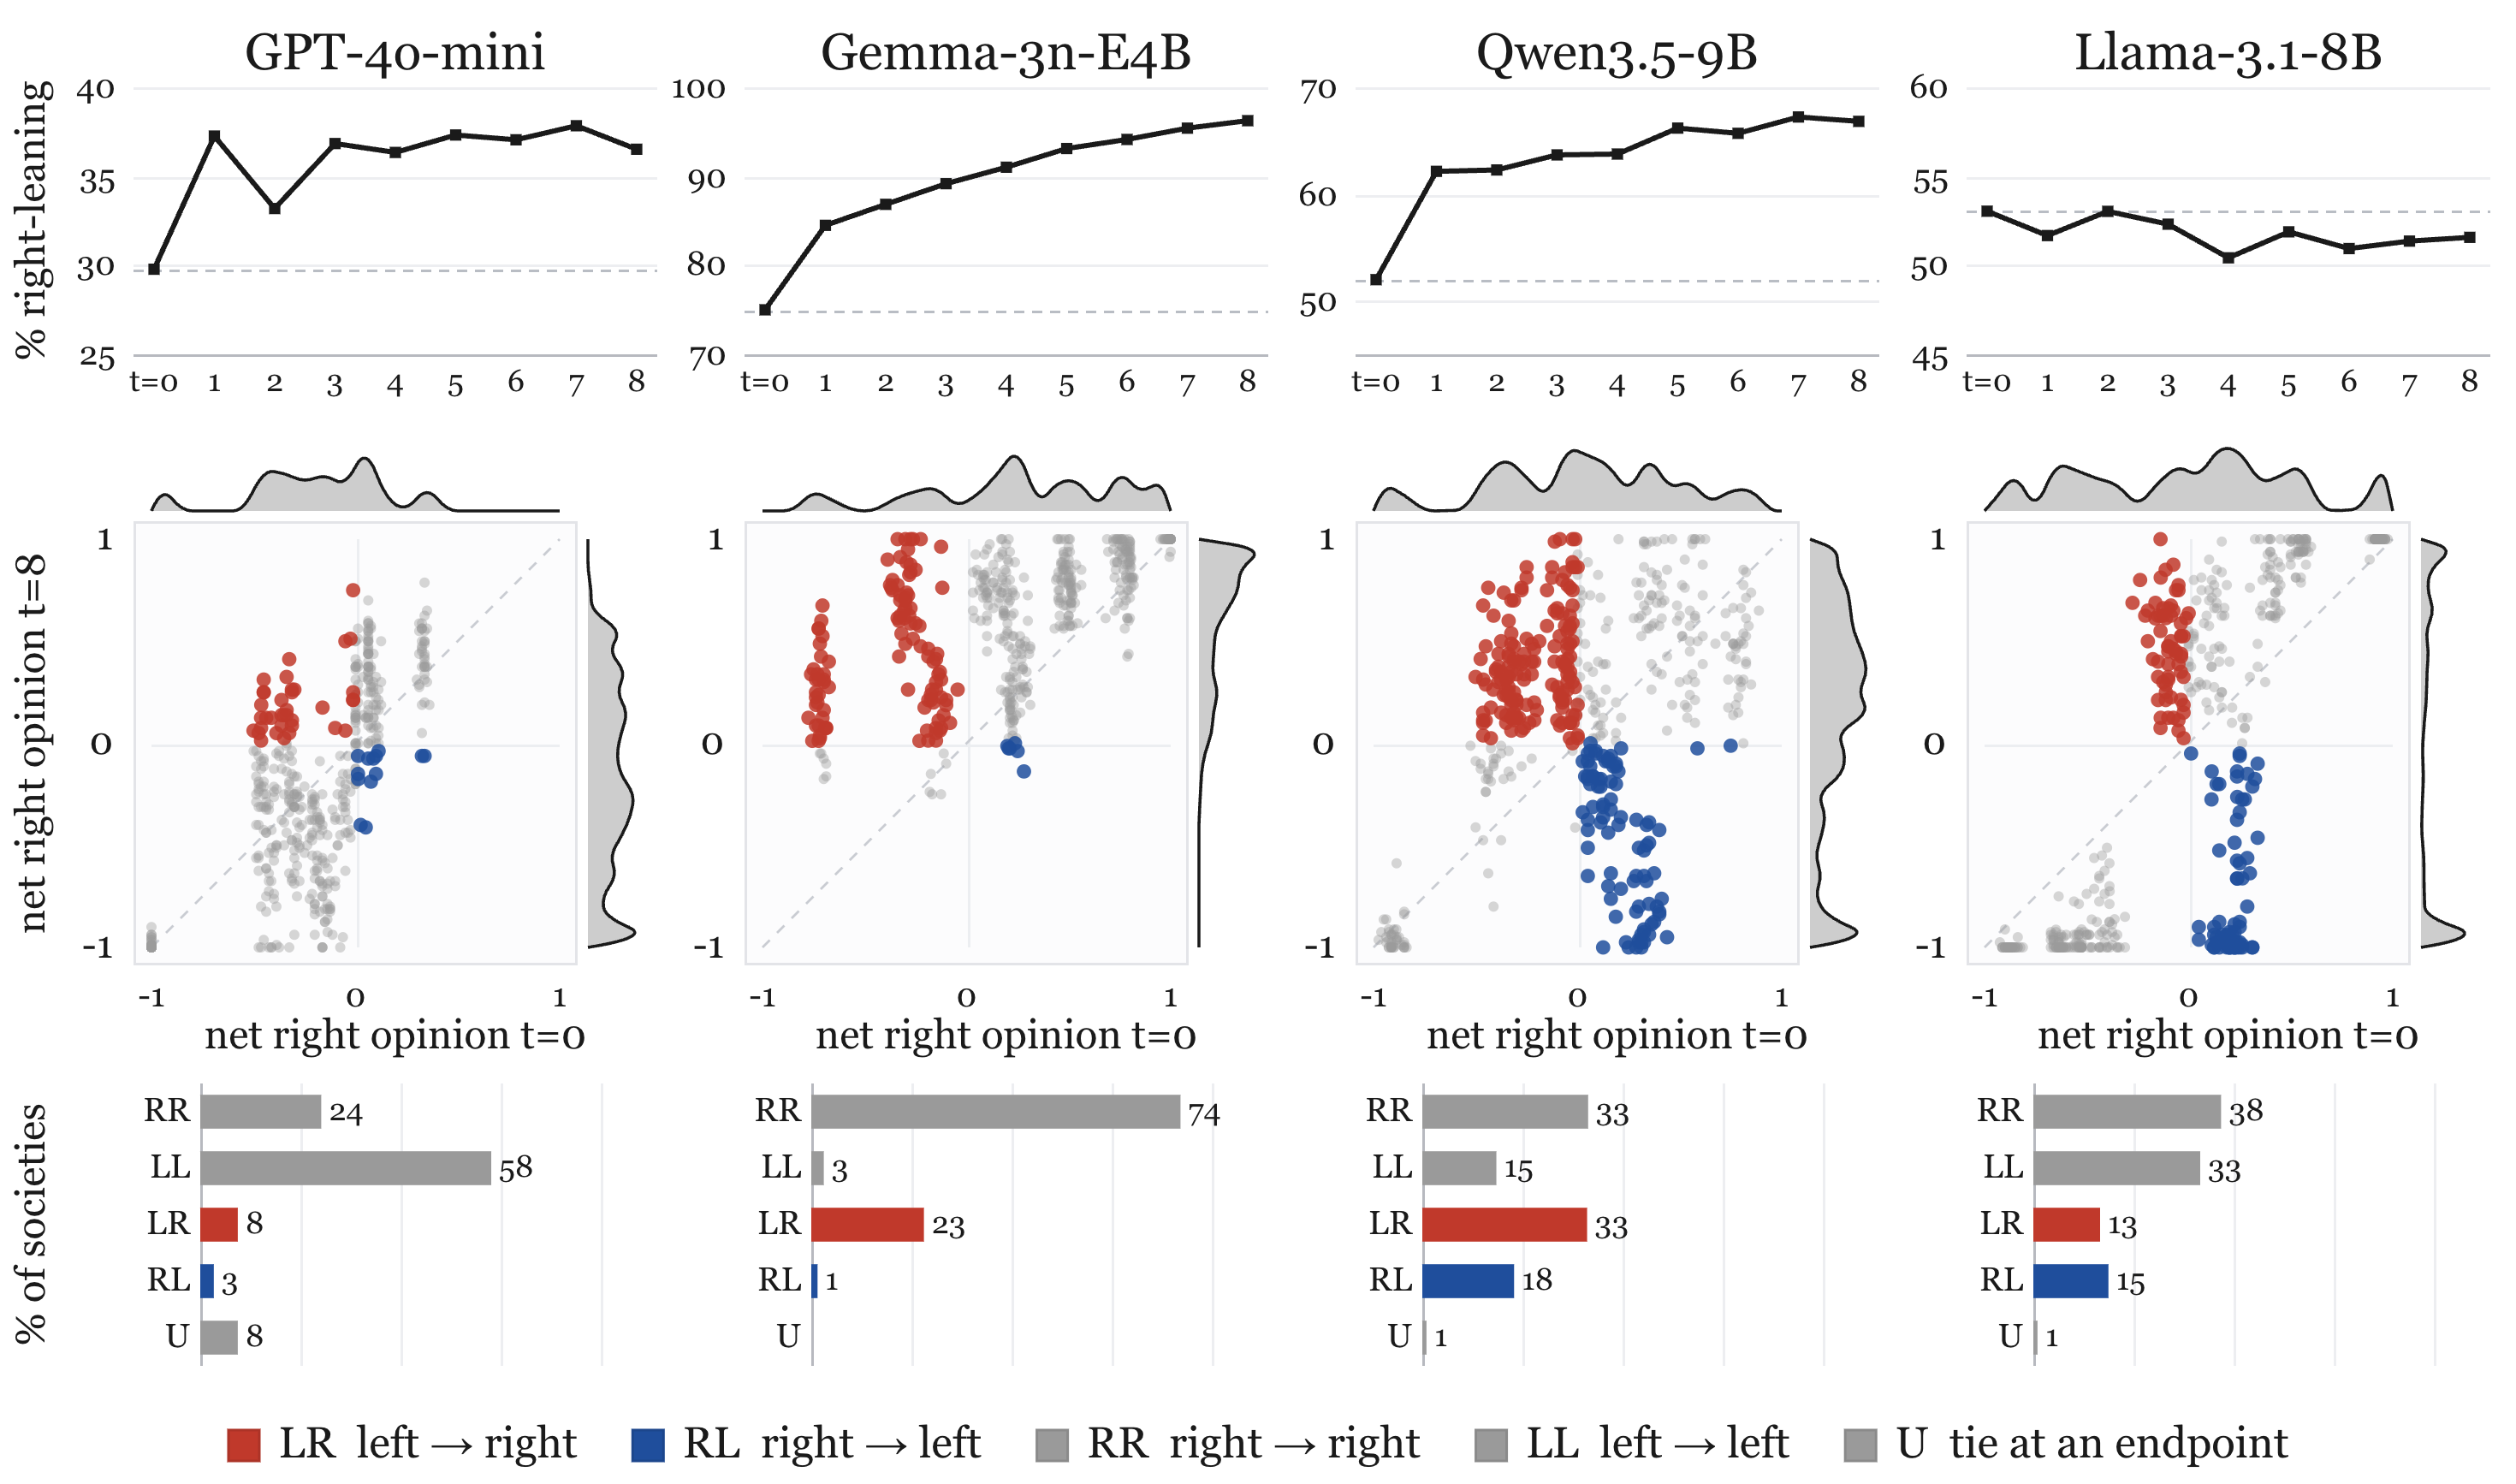
\includegraphics[width=0.99\textwidth]{main/Figures/apx_04_political_lean.png}
        \caption{\textit{Political lean.} How opinions move along the left--right axis on the political statements ($1,920 = 4 \times 12 \times 10 \times 4$ groups from subjective questions only, from signed random graphs and the square and triangular lattices, over both the training- and test-set questions). The statement set is label-balanced (randomly sampling 6 statement with agree leaning left and 6 statement with agree leaning right from Table \ref{tab:political-stance}) so that uniform answer-label bias cancels and does not register as political drift. In a group trajectory, an opinion is represented as right-leaning if net opinion has the same sign as right-leaning opinion. To define which sign a right-leaning opinion has, we labeled the political leaning of agreeing with the statements in our dataset as shown in Table \ref{tab:political-stance}. \emph{Row 1:} $y$-axis: percentage of group trajectories, where the net opinion $n(t)$ has the right-leaning sign at round $t$. $x$-axis: timesteps. \emph{Row 2:} Each point represents a group trajectory, which is plotted based on its initial ($t=0$, $x$-axis) and final ($t=8$, $y$-axis) net opinion $n(t)$ multiplied by the sign of the right-leaning opinion of the questions to get \textit{net right opinion}: $n(t) \cdot y_{r}$, where $y_{r} \in \{-1, +1\}$ denotes the sign of the right-leaning opinion. \emph{Row 3:} Groups switch between being left-leaning and right-leaning at $t=0$ and $t=8$. LL (left$\to$left), LR (left$\to$right), RL (right$\to$left), RR (right$\to$right), and U (undecided, $50\text{-}50$ tie at $t=0$ or $t=8$). The two transition categories LR and RL are highlighted.}
\label{fig:3_Observations_politicallean}
\end{figure}

\subsection{Political Lean of Interacting Agents}\label{apdx:political_lean}



In Section~\ref{sec:truth_seeking}, we explored the truth seeking on objective questions. Here, we present analogous results for subjective questions with a political lean. We labeled the political leaning of each of the political statements in our dataset as shown in Table \ref{tab:political-stance}. In Figure~\ref{fig:3_Observations_politicallean}, we track the fraction of communities whose net opinion sits on the right-leaning side. Three of the four models drift to the right over the eight rounds: Gemma-3n-E4B moves from $75\%$ to $96\%$, Qwen3.5-9B from $52\%$ to $67\%$, and GPT-4o-mini from $30\%$ to $37\%$. Llama-3.1-8B-Instruct is the exception and stays near its starting value of $53\%$, ending marginally lower. The transition counts in the third row make the same point at the level of individual trajectories. Left$\to$right switches outnumber right$\to$left switches by $23\%$ to $1\%$ for Gemma-3n-E4B, $33\%$ to $18\%$ for Qwen3.5-9B, and $8\%$ to $3\%$ for GPT-4o-mini, while Llama-3.1-8B-Instruct is close to symmetric ($13\%$ versus $15\%$). Note that GPT-4o-mini begins strongly left-leaning ($30\%$ right at $t=0$) and still moves rightward under interaction, so the initial distribution of opinions and the direction of drift are separate properties of a community.


\definecolor{leanleft}{HTML}{214E98}   %
\definecolor{leanright}{HTML}{BE3D31}  %

\newcommand{\lleft}{\textcolor{leanleft}{left}}
\newcommand{\lright}{\textcolor{leanright}{right}}
\newcommand{\lnone}{---}

\begin{table}[htbp]
\centering
\small
\setlength{\tabcolsep}{4pt}
\begin{tabularx}{\textwidth}{@{}r l l X l l l@{}}
\toprule
\# & QID & Split & Question & Pole $+$ & Pole $-$ & Agree leans \\
\midrule
1  & \texttt{political\_stance\_0}   & train & Student loan debt should be forgiven by the government     & Agree & Disagree & \lleft  \\
2  & \texttt{political\_stance\_4}   & train & Protest permits infringe on the right to peaceful assembly  & Agree & Disagree & \lnone  \\
3  & \texttt{political\_stance\_11}  & train & Private equity firms harm the companies they acquire        & Agree & Disagree & \lleft  \\
4  & \texttt{political\_stance\_17}  & train & Mandatory vaccination violates bodily autonomy              & Agree & Disagree & \lright \\
5  & \texttt{political\_stance\_62}  & train & Farm subsidies distort markets and should be phased out     & Agree & Disagree & \lright \\
6  & \texttt{political\_stance\_68}  & train & Sanctuary city policies undermine federal immigration law   & Agree & Disagree & \lright \\
7  & \texttt{political\_stance\_72}  & train & Homeschooling should face stricter government oversight     & Agree & Disagree & \lleft  \\
8  & \texttt{political\_stance\_76}  & train & Patent terms should be shortened to encourage innovation    & Agree & Disagree & \lnone  \\
9  & \texttt{political\_stance\_104} & train & Peaceful protest is more effective than civil disobedience  & Agree & Disagree & \lnone  \\
10 & \texttt{political\_stance\_145} & train & Billionaires should not exist in a just society             & Agree & Disagree & \lleft  \\
\addlinespace
11 & \texttt{political\_stance\_156} & test  & Financial transaction taxes would reduce market volatility  & Agree & Disagree & \lleft  \\
12 & \texttt{political\_stance\_231} & test  & Foreign aid spending weakens domestic economic priorities   & Agree & Disagree & \lright \\
13 & \texttt{political\_stance\_232} & test  & The US should maintain military bases around the world      & Agree & Disagree & \lright \\
14 & \texttt{political\_stance\_254} & test  & Stricter gun control laws would reduce violent crime rates  & Agree & Disagree & \lleft  \\
15 & \texttt{political\_stance\_266} & test  & Breaking up big tech companies would increase innovation    & Agree & Disagree & \lnone  \\
16 & \texttt{political\_stance\_353} & test  & Campus speech codes violate First Amendment principles      & Agree & Disagree & \lright \\
17 & \texttt{political\_stance\_361} & test  & NATO expansion provokes conflict and should be halted       & Agree & Disagree & \lnone  \\
18 & \texttt{political\_stance\_363} & test  & Defense spending should be reduced to fund social programs  & Agree & Disagree & \lleft  \\
19 & \texttt{political\_stance\_382} & test  & Critical race theory should be taught in K--12 schools      & Agree & Disagree & \lleft  \\
20 & \texttt{political\_stance\_393} & test  & Nuclear power is essential for achieving clean energy goals & Agree & Disagree & \lnone  \\
\bottomrule
\end{tabularx}
\caption{Political stance items, with train/test split and the direction the ``Agree'' pole leans (\lleft{} / \lright{} / neutral).}
\label{tab:political-stance}
\end{table}

\subsection{Label Bias}
\begin{figure}[h!]
    \centering
    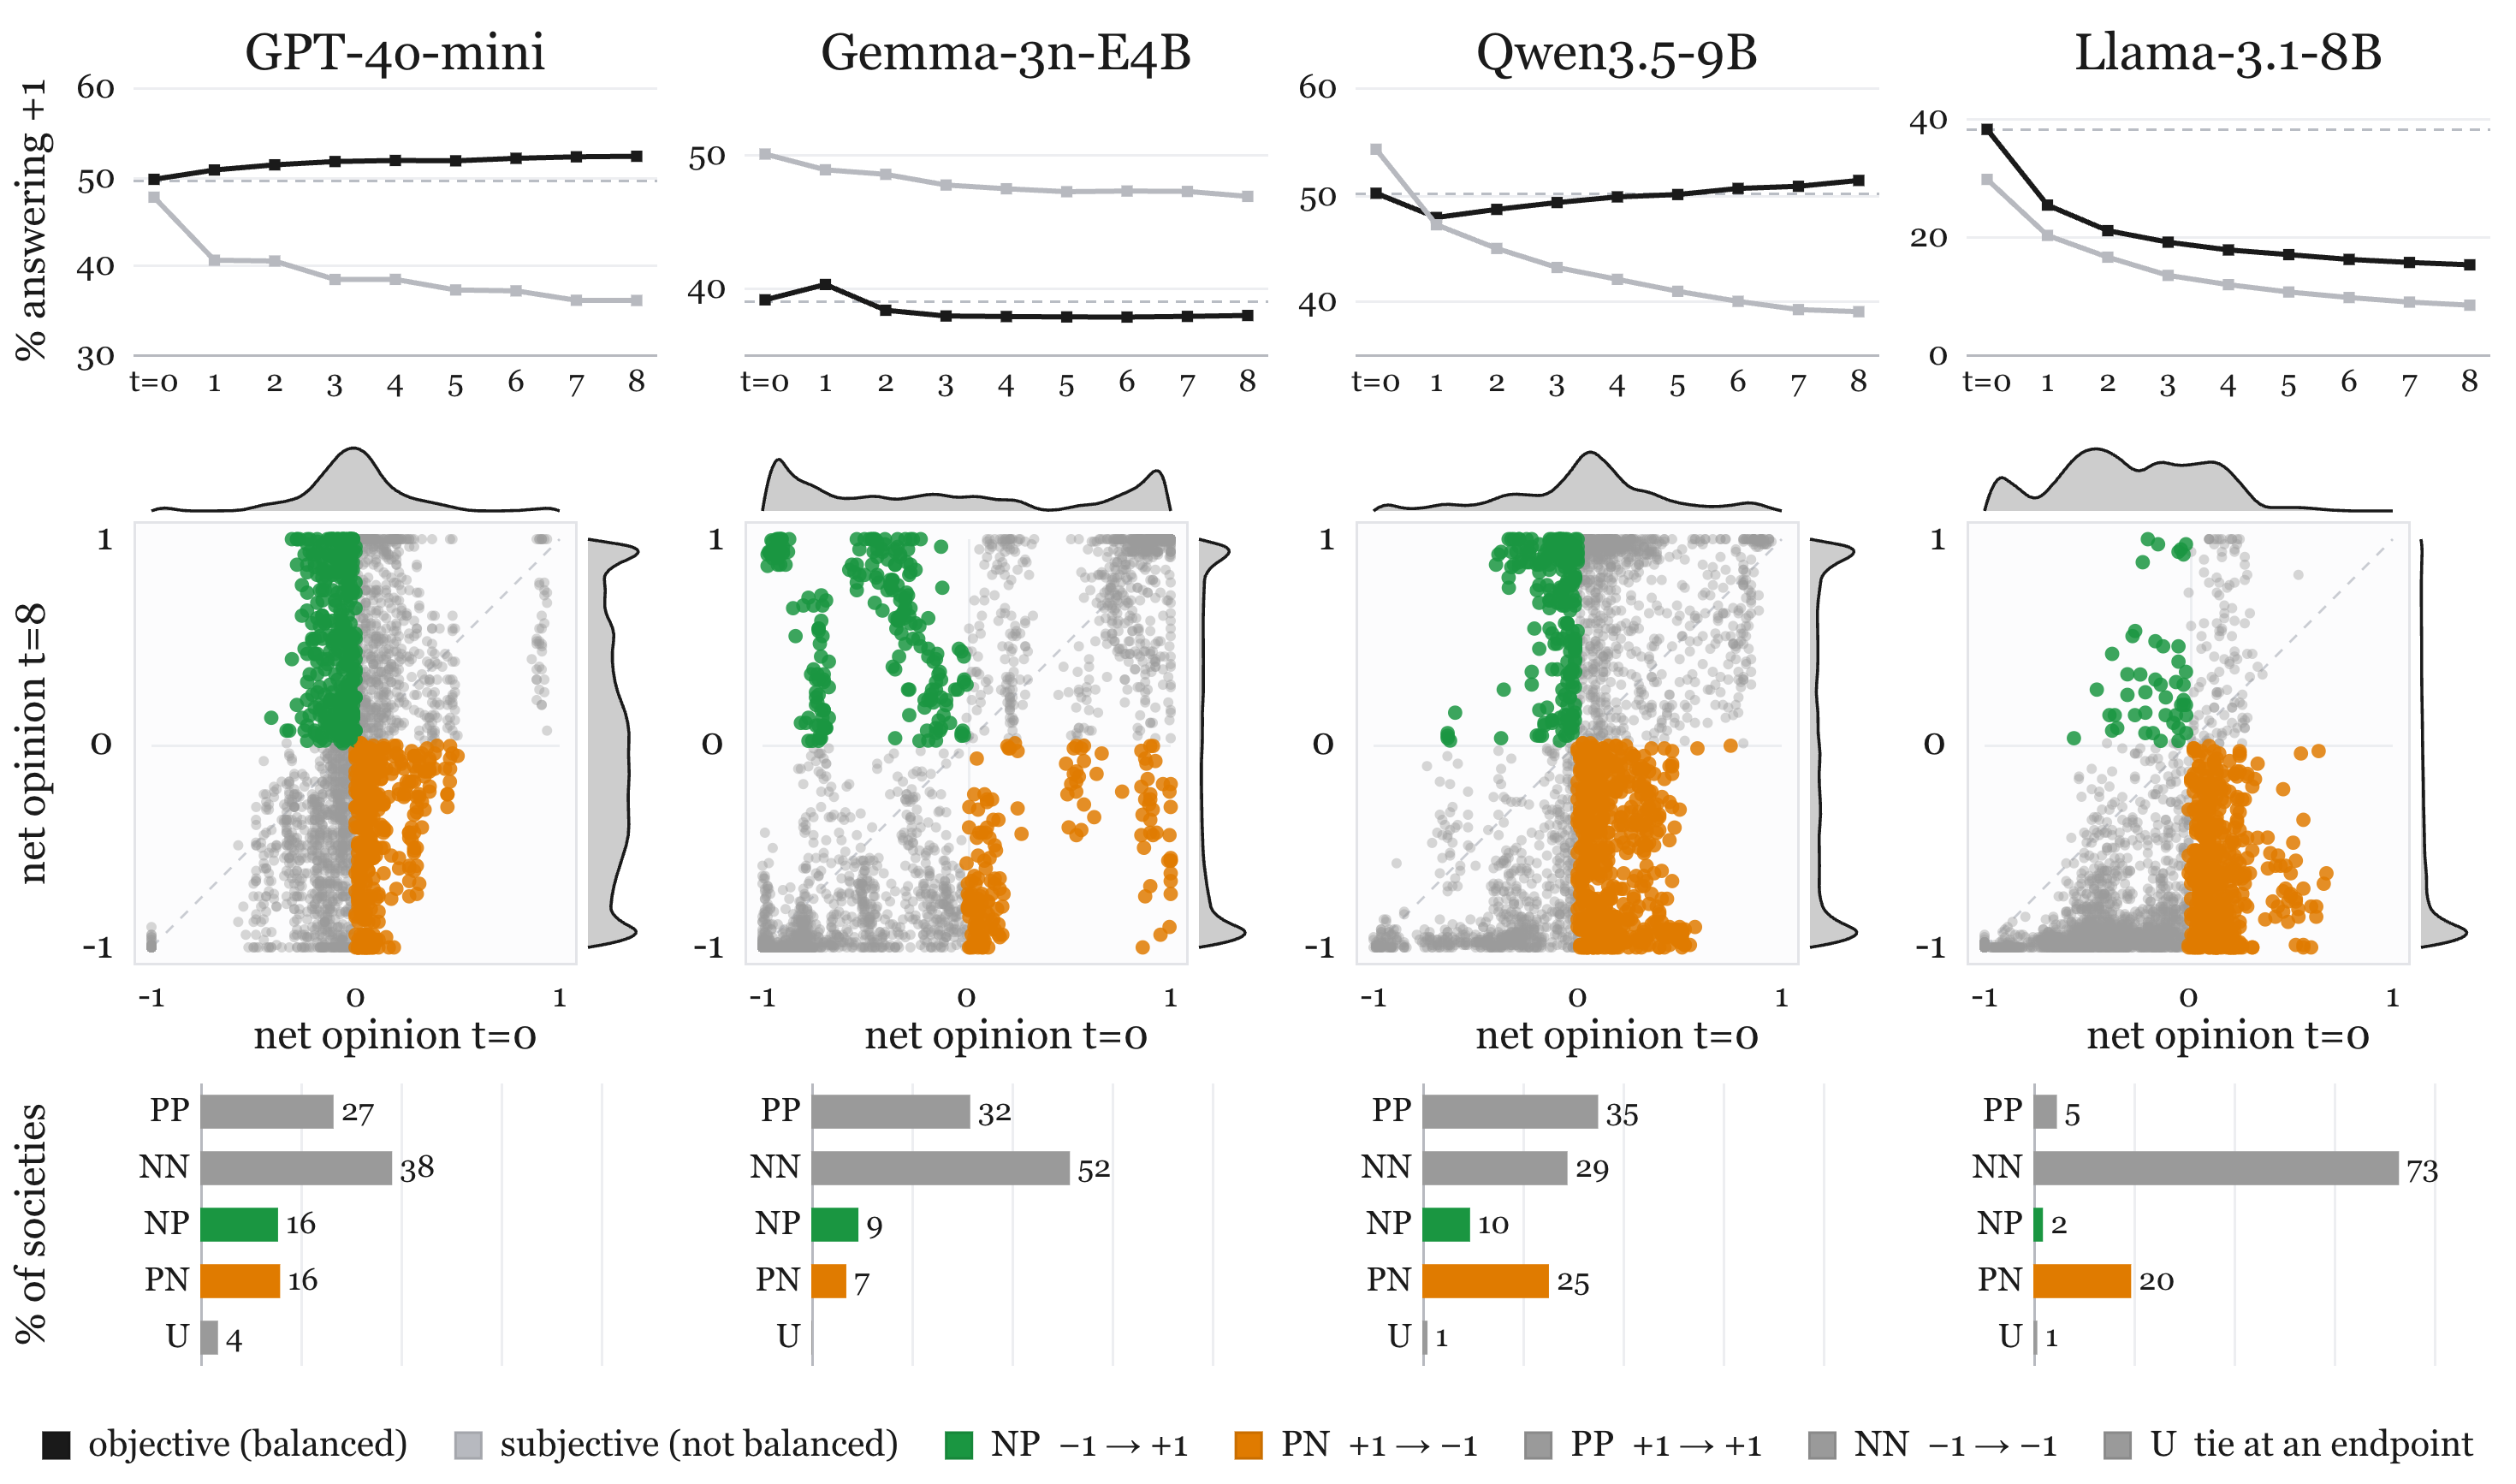
\includegraphics[width=0.99\textwidth]{main/Figures/apx_05_label_bias.png}
            \caption{\textit{Label Bias.} How opinions move along the $+1 / -1$ axis over the run ($9,600$ groups from both objective and subjective questions, spanning signed random graphs and the square and triangular lattices, over both the training- and test-set questions). \emph{Row 1:} $y$-axis: percentage of group trajectories, where the net opinion $n(t)$ has positive sign at round $t$. $x$-axis: timesteps. \emph{Row 2:} Each point represents a group trajectory, which is plotted based on its initial ($t=0$, $x$-axis) and final ($t=8$, $y$-axis) net opinion $n(t)$  \emph{Row 3:} Groups switch between $+1$ and $-1$ at $t=0$ and $t=8$. PP (positive$\to$positive), NN (negative$\to$negative), NP (negative$\to$positive), PN (positive$\to$negative), and U (undecided, $50\text{-}50$ tie at $t=0$ or $t=8$). The two transition categories NP and PN are highlighted.}
\label{fig:3_Observations_bias}
\end{figure}

\textit{Label Bias.} A community can also drift toward an answer option irrespective of what that option says (Figure~\ref{fig:3_Observations_bias}). Because the objective questions are label balanced, with the correct answer being $+1$ as often as $-1$, a change in the fraction of agents answering $+1$ over the course of a run cannot be attributed to truth seeking. However, we still observe such a change for Llama-3.1-8B-Instruct, with the fraction answering $+1$ falling from $39\%$ to $16\%$.


\clearpage
\subsection{Thresholds for Characteristic Regimes}\label{apdx:mode_thresholds}

\begin{table}[h!]
\centering
\begin{tabular}{llcc}
\toprule
 & & \multicolumn{2}{c}{Threshold} \\
\cmidrule(lr){3-4}
Regime & Model & Conviction $c^\star$ & Net opinion $n^\star$ \\
\midrule
\multirow{4}{*}{Objective}
              & GPT-4o-mini   & 0.910 & 0.475 \\
              & Gemma-3n-E4B  & 0.940 & 0.994 \\
              & Qwen3.5-9B    & 0.790 & 0.913 \\
              & Llama-3.1-8B    & 0.740 & 0.913 \\
\midrule
\multirow{4}{*}{Subjective}
              & GPT-4o-mini   & 0.960 & 0.375 \\
              & Gemma-3n-E4B  & 0.910 & 0.725 \\
              & Qwen3.5-9B    & 0.820 & 0.600 \\
              & Llama-3.1-8B    & 0.950 & 0.963 \\
\bottomrule
\end{tabular}
\caption{\textit{Selected thresholds for Figure \ref{fig:3_Observations_modes}}. For each model--regime row, the
\emph{conviction threshold} $c^\star$ is defined as the $1/3$ quantile of conviction,
pooled across all episodes, graphs, and rounds; communities with $c(t)<c^\star$ are
classified as \emph{indifferent}. The \emph{net-opinion threshold} $n^\star$ is then
defined as the median of $|n(t)|$ among the remaining ``committed'' communities and
applied symmetrically as $\pm n^\star$ to distinguish \emph{polarization}
($|n(t)|\le n^\star$) from \emph{consensus} ($|n(t)|>n^\star$). Both thresholds are
reported on their native ranges, $c\in[0,1]$ and $|n|\in[0,1]$.}
\label{tab:mode_thresholds}
\end{table}

\subsection{Rare Group Trajectories}\label{apdx:rare_macrostates}

\begin{figure}[h]
    \centering
    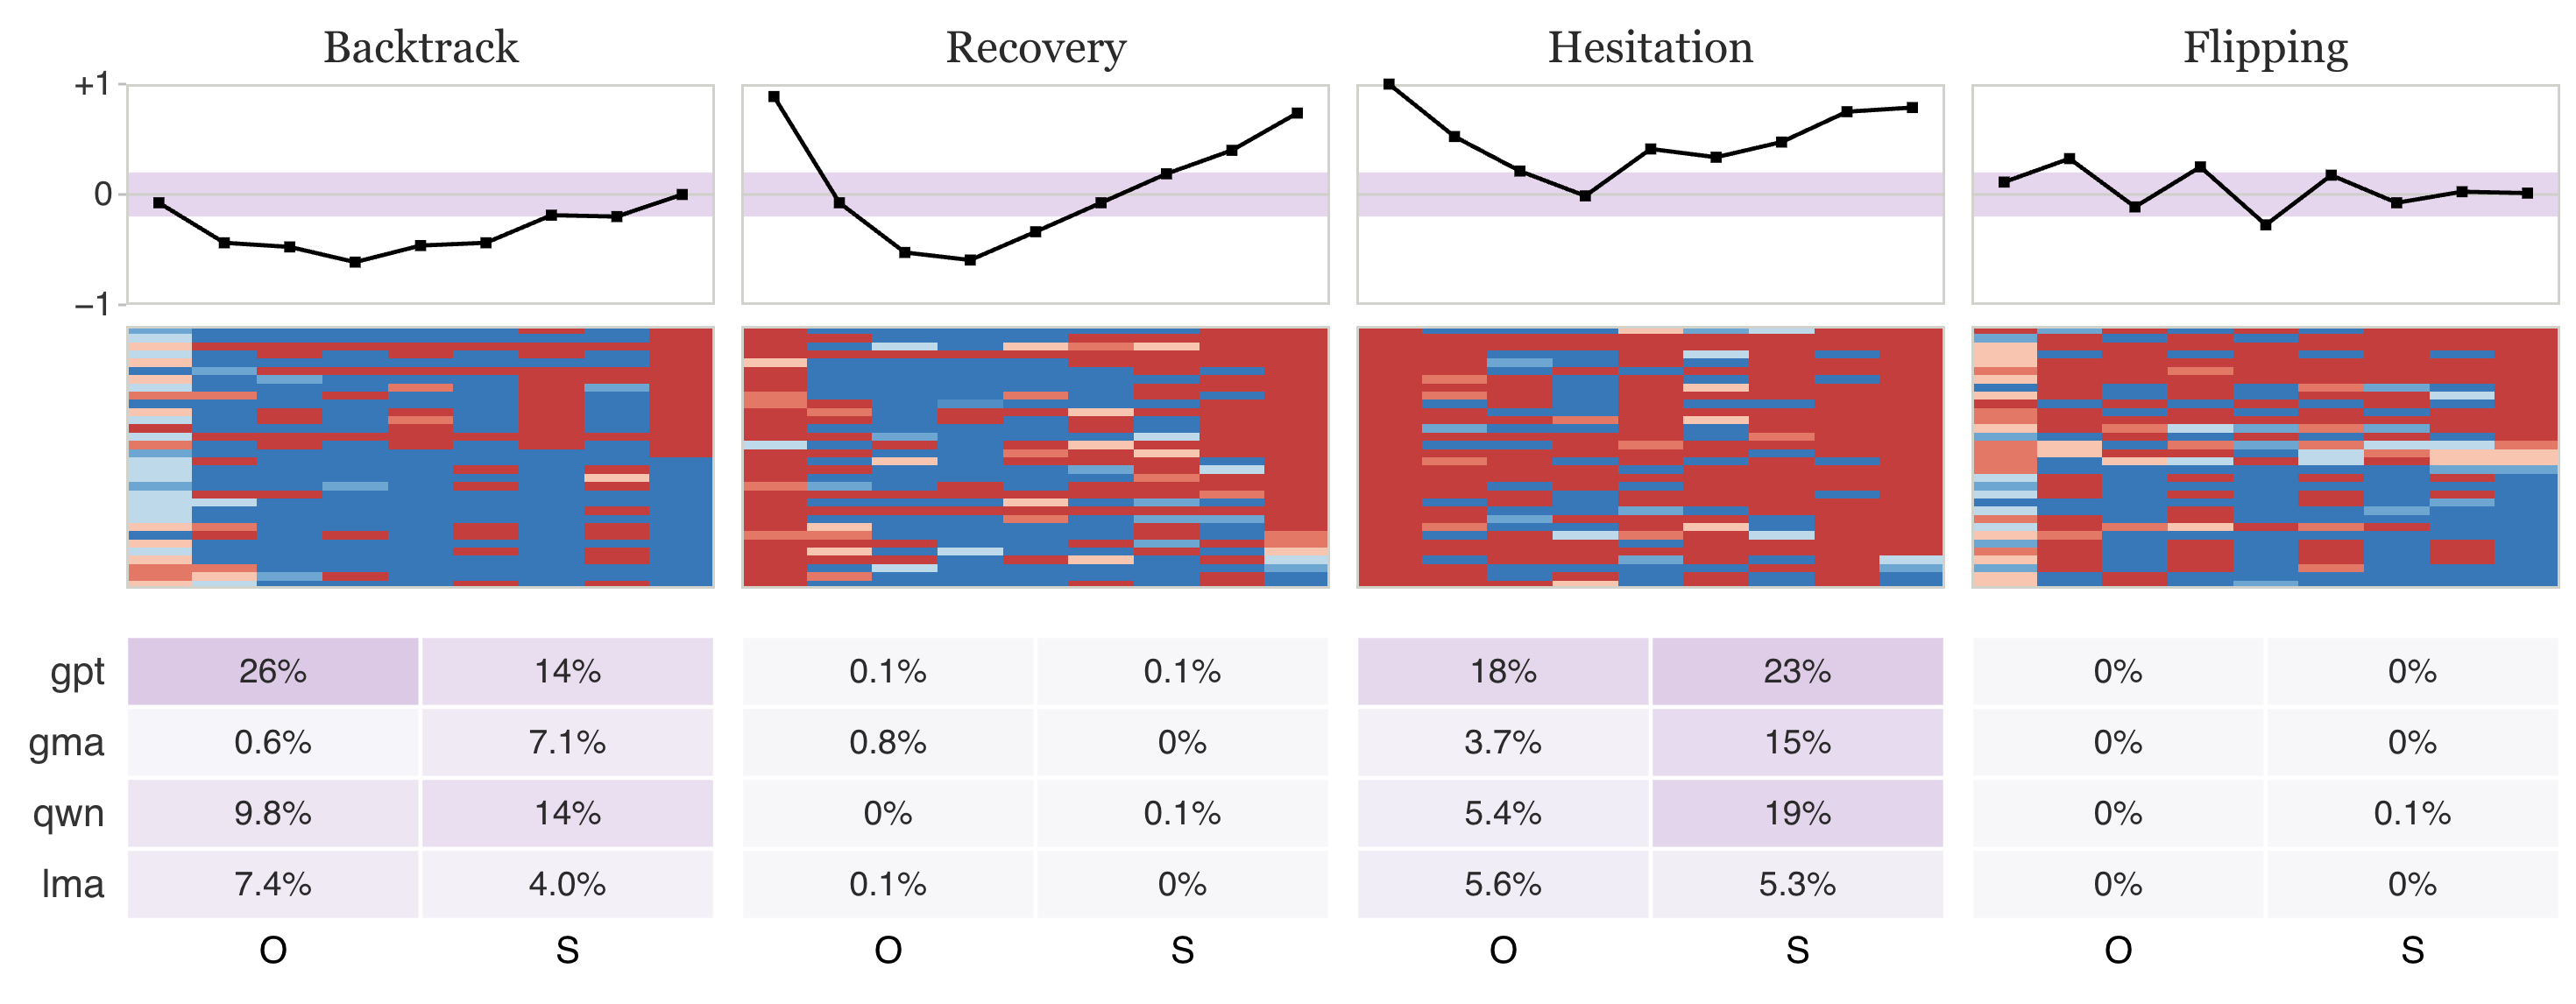
\includegraphics[width=0.99\textwidth]{main/Figures/apx_06_rare_macrostates.png}
\caption{\textit{Rare and non-monotone group trajectories.}
Groups whose net opinion \emph{reverses
direction} mid-run, which a first-vs-last-round classification cannot distinguish. Same setup as
Figure ~\ref{fig:macrostates}. A \emph{strong majority} denotes a round with absolute net opinion $|n(t)| \geq 0.5$, which is beyond the
split band $ \le \delta = 0.2$.}
\label{fig:rare_macrostates}
\end{figure} 

\emph{Backtrack}: A split community (absolute net opinion in $\pm 0.2$ split band) first develops a strong majority (absolute net opinion $\geq 0.5$) before relaxing back toward a split. \emph{Recovery}: A strong majority (absolute net opinion $\geq 0.5$) reverses to the opposite side before returning to its original position. \emph{Hesitation}: A strong majority weakens almost to a split, then re-consolidates on the same side. \emph{Flipping}: The majority repeatedly changes sides during the simulation.


\subsection{Effect of Communication Networks on  Trajectories}\label{apdx:communication_effect}

\begin{figure}[h]
    \centering
    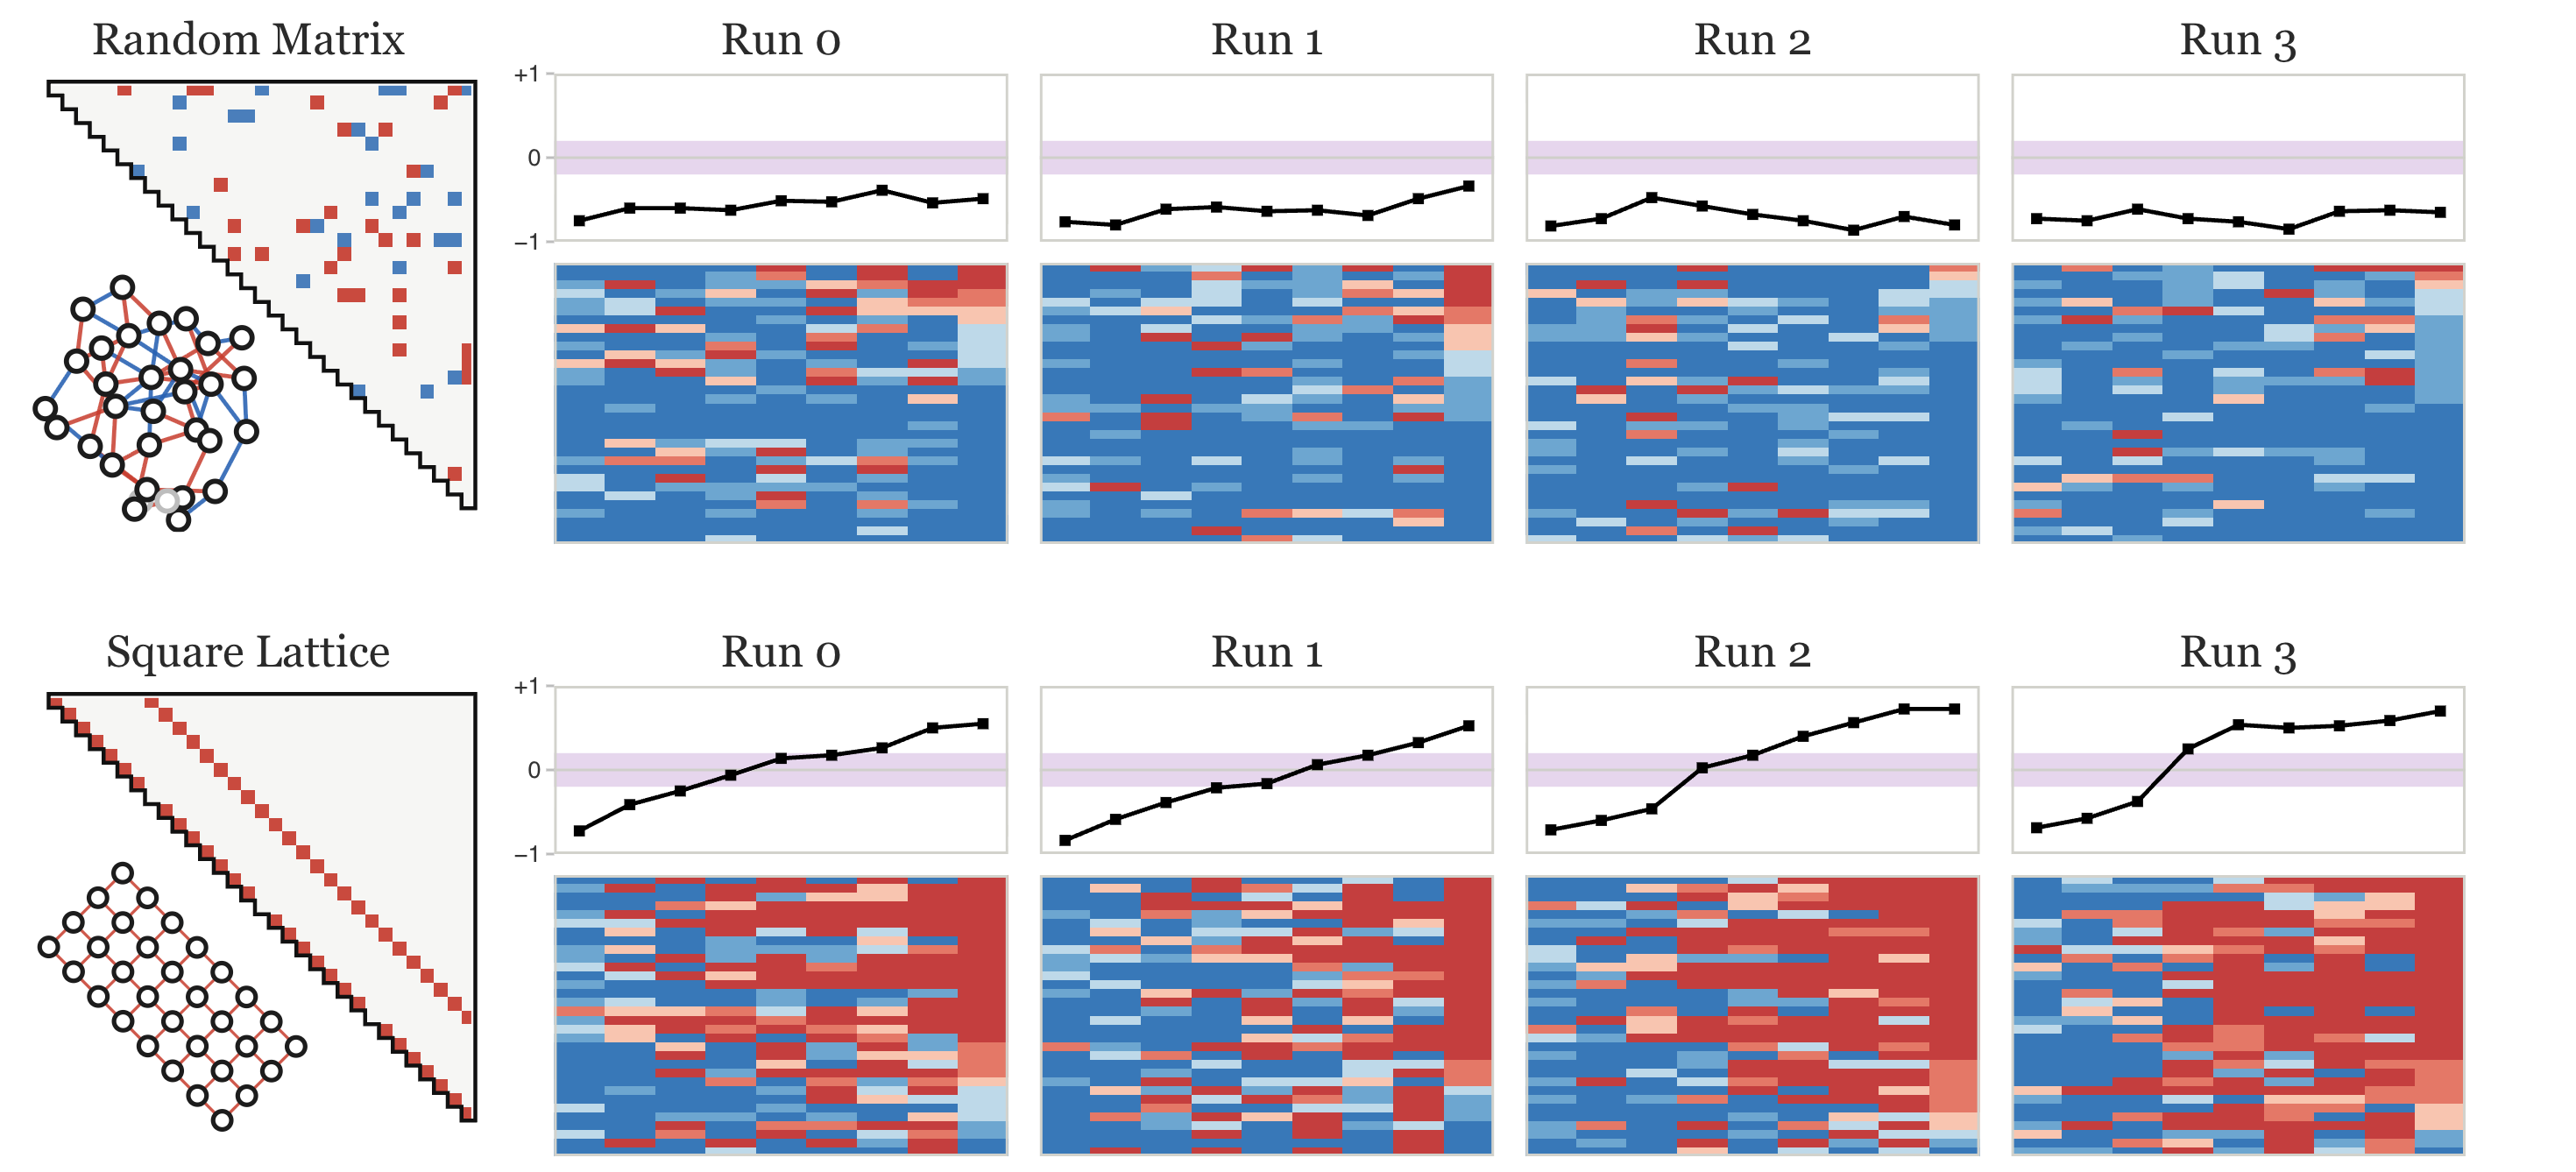
\includegraphics[width=0.99\textwidth]{main/Figures/apx_07_communication_networks.png}
\caption{\textit{Different communication networks can cause differences in trajectories.} Four episodes (labeled as runs 0-3) on the same question under two different social graphs: a random matrix (\emph{top}) and a square lattice (\emph{bottom}). For each graph, the left panel shows the couplings $J$ as a heatmap in the upper triangle and as a node-link diagram below it, and each of the four runs shows the net opinion $n(t)$ over rounds (\emph{line plot at the top}) together with the group trajectory (\emph{heatmap at the bottom}). Under the random matrix the community stays on its initial side across all four runs, while under the square lattice it crosses the split band and settles on the opposite side in all four runs. This is not a common situation, but social graphs can cause consistent differences between how group trajectories evolve when answering the same question. In other words, the social connections carry information about where will the community end up, even before any messages are exchanged.}
\label{fig:communication_networks}
\end{figure}



\section{Method Details}\label{apdx:method}
\subsection{Local Update Rule}\label{apdx:discrete-updates}

This appendix derives the logistic update rule of Section~\ref{sec:method} from the energy function and assuming the Boltzmann distribution. For energy-based models of this form, the Boltzmann distribution is the stationary distribution of the standard stochastic relaxation with asynchronous updates, which is a construction used throughout the Ising literature and its applications to neural and social systems
\citep{glauber1963,hopfield1982neural,brock2001,castellano2009}. Our derivation uses only the single-agent conditional distribution induced by this measure as a starting point. Appendix ~\ref{apdx:async_update} and Appendix ~\ref{apdx:continuous-extension} treat the asynchronous case, where Boltzmann distribution is the stationary distribution of the dynamics.


\textit{Local Field.} Let $s_{i} \in \{+1,-1\}$ be the opinion of agent $i$. Fixing all opinions other than $s_i$, the energy
\[
E(s) \;=\; -\frac{1}{2}\sum_{i=1}^n \sum_{j=1}^n J_{ij}\,s_i s_j \;-\; \sum_{i=1}^n g_i\,s_i
\]
splits into a part that depends on $s_i$ and a part that does not,
\[
E(s) \;=\; -\,s_i f_i \;+\; C,
\qquad
f_i \;=\; \sum_{j\neq i} J_{ij}\,s_j \;+\; g_i ,
\]
where $C$ collects every term independent of $s_i$. The factor $\tfrac12$ disappears because
$J = J^{\top}$ with zero diagonal, so $s_i$ appears twice in the double sum, once in row $i$
and once in column $i$. We call $f_i$ the \emph{local field} on agent $i$: the total pull that
its neighbors and its own predisposition exert on it.


Under the Boltzmann distribution $P(s) \propto e^{-\beta E(s)}$, the probability that $s_i = +1$ conditional on the rest of the group $s_{-i}$ is obtained by normalizing over the two
values $s_i$ can take,
\[
P(s_i = +1 \mid s_{-i})
\;=\; \frac{e^{-\beta E(s_i=+1)}}{e^{-\beta E(s_i=+1)} + e^{-\beta E(s_i=-1)}} .
\]
Substituting $E(s) = -s_i f_i + C$ and cancelling the common factor $e^{-\beta C}$ gives
\[
P(s_i=+1\mid s_{-i})
= \frac{e^{\beta f_i - \beta C}}{e^{\beta f_i - \beta C} + e^{-\beta f_i - \beta C}}
= \frac{e^{\beta f_i}}{e^{\beta f_i} + e^{-\beta f_i}}
= \frac{1}{1 + e^{-2\beta f_i}}
= \sigma\!\left(2\beta f_i\right),
\]
and
\[
P(s_i=+1\mid s_{-i})
\;=\; \sigma\!\Big(2\beta \big(\textstyle\sum_{j\neq i} J_{ij}\,s_j + g_i\big)\Big)
\;=\; \sigma\!\left(\tilde\beta \sum_{j} J_{ij}\,s_j(t) + \tilde g_i\right),
\]
where the last step absorbs the factor of $2$ into the coupling, $\tilde\beta = 2\beta$, and
writes $\tilde g_i = 2\beta g_i$ for the rescaled local bias. The two are not separately
identified from opinion data alone: only the products $\tilde\beta$ and $\tilde g_i$ enter the
likelihood, which is why we fit $\tilde\beta$ and $\tilde g_i$ directly and report the fitted
model as sitting at temperature $\mathcal{T} = 1$ (Section~\ref{sec:results_temperature}). An agent's
next opinion is therefore a logistic function of (a) the peer pressure
$\sum_j J_{ij}s_j(t)$ flowing in along the signed graph, scaled by $\tilde\beta$, and (b) an
intrinsic field $\tilde g_i$ encoding the leaning of agent $i$'s persona on this question in
the absence of any peer influence. We omit $\;\tilde{\cdot}\;$ and use $\beta$ and $g_i$ parameters in the main text for simplicity.

\textit{Synchronous Updates.} The observed data record one opinion per agent per round, with
all agents polled at the same round boundary, so we apply the rule synchronously: every agent's
next opinion is drawn from the law above evaluated at the \emph{current} configuration
$s(t)$, and all of them are updated at once to form $s(t+1)$. Appendix~\ref{apdx:continuous-extension} relaxes it by letting agents update at
independent random times, following  \citet{glauber1963}.

\subsection{Continuous Extension}\label{apdx:continuous-extension}

The dynamics of Appendix~\ref{apdx:discrete-updates} assume that all agents update their
opinions synchronously at discrete time steps. We now relax this assumption by introducing a
continuous-time model in which agents revise their opinions independently at random times, as in \citet{glauber1963}.

\subsubsection{Flip Rate}

\textit{Update Rate.} Agent $i$ reconsiders its opinion during a small time window $\mathrm dt$
with probability $\mathrm dt/\tau$, independently of everything that has happened before. We call $1/\tau$ the agent's update rate. Every agent has its own update mechanism, running independently at the rate $1/\tau$.

\textit{Probability of a Flip.} For simplicity, in this section, we move $\beta$ inside $f_i$ and define $f_i \;=\; \beta  \sum_{j\neq i} J_{ij}\,s_j \;+\; g_i$. Note that the probability that $s_i$ is $+1$ is $P(s_i = +1) = \sigma(2f_i)$ and the
probability that $s_i$ is $-1$ is $P(s_i = -1) = 1 - \sigma(2f_i) = \sigma(-2f_i)$. Then, given
the current state is $+1$, the probability of a flip is $\sigma(-2f_i)$, and given the current
state is $-1$, the probability of a flip is $\sigma(2f_i)$. We can write the probability of a
flip more compactly as
\(
P(\text{flip}) = \sigma(-s_i\,2f_i)
\).

\textit{Flip rate $=$ Update Rate $\times$ Probability of a Flip.} Now, we combine the update
rate with the probability of a flip to obtain the flip rate. Using
$\sigma(-2x) = \tfrac{1}{2}\big(1 - \tanh x\big)$ and $\tanh(s_i f_i) = s_i \tanh f_i$, we get
\(
P(\text{flip}) = \sigma(-s_i 2f_i) = \tfrac{1}{2}\big(1 - s_i \tanh f_i\big).
\) The flip rate $w_i$ is the update rate times the flip probability,
\[
w_i(s) = \frac{1}{\tau}\,\sigma(-s_i 2f_i)
= \frac{1}{2\tau}\big(1 - s_i \tanh f_i\big)
= \frac{1}{2\tau}\big(1 - s_i \langle s_i\rangle_c\big).
\]

\subsubsection{Master Equation}

Now, we introduce the master equation, which describes the probability flux between states and
is derived from the conservation of probability mass. At any given time, the system must occupy
one of the possible states in its state space. Consequently, the total probability over all
states must remain equal to one. This implies that probability mass cannot be created or
destroyed. It can only flow from one state to another. Therefore, for each state, the rate of change of its probability is determined by the balance between the probability flux entering the state and the probability flux leaving it. The master equation formalizes this balance by equating the net change in probability to the total inflow minus the total outflow of probability mass.

\textit{Flip operator $\mathcal{F}$.} Define $\mathcal{F}_i s$ as state $s$ with agent $i$ flipped,
\(
\mathcal{F}_i s = [\,s_1,\ \ldots,\ -s_i,\ \ldots,\ s_n\,].
\)
\textit{Master Equation.} The probability of being at state $s$ changes based on the difference
between the inflow into and outflow out of state $s$,
\[
\frac{d}{dt}P(s,t) = \sum_{i=1}^{n}
\underbrace{w_i(\mathcal{F}_i s)\,P(\mathcal{F}_i s, t)}_{\text{inflow into } s}
- \underbrace{w_i(s)\,P(s,t)}_{\text{outflow out of } s}.
\]
This is a probability-flow equation expressing conservation of probability mass in the system,
where $w_i(\mathcal{F}_i s)$ is the probability that $i$ flips at $\mathcal{F}_i s$, and $P(\mathcal{F}_i s, t)$ is the
probability mass allocated to $\mathcal{F}_i s$. The inflow into $s$ is $w_i(\mathcal{F}_i s)\times P(\mathcal{F}_i s, t)$
and the outflow out of $s$ is $w_i(s)\times P(s,t)$, where
\[
w_i(s) = \frac{1}{2\tau}\big(1 - s_i \tanh f_i\big),
\qquad
w_i(\mathcal{F}_i s) = \frac{1}{2\tau}\big(1 - (-s_i)\tanh f_i\big)
= \frac{1}{2\tau}\big(1 + s_i \tanh f_i\big).
\]

\subsubsection{Mean-Field ODE}

The master equation tracks the full distribution $P(s,t)$ over all $2^n$ configurations, which
is intractable to follow directly. Instead, we track only the quantity we care about: each
agent's opinion, 
$m_i(t) = \langle s_i(t)\rangle = \sum_s s_i\,P(s,t)$, which is between
$-1$ (the agent is surely $-1$) and $+1$ (surely $+1$).

We can derive how $m_i$ evolves directly from the master equation. The only events that change $s_i$ are flips of agent $i$ itself. Each flip sends $s_i \mapsto -s_i$, a change of $-2s_i$, and these flips occur at rate $w_i(s)$. Averaging this
instantaneous change over the distribution gives
\[
\frac{d m_i}{dt}
= \big\langle -2\,s_i\,w_i(s)\big\rangle
= -\frac{1}{\tau}\big\langle s_i\big(1 - s_i \tanh f_i\big)\big\rangle
= -\frac{1}{\tau}\Big(\langle s_i\rangle - \big\langle \tanh f_i\big\rangle\Big),
\]
where the last step uses $s_i^2 = 1$. This relation is exact; however, the average
$\langle \tanh f_i\rangle$ is intractable to compute.

\textit{Mean-field approximation.} To make this quantity tractable, we make the mean-field approximation. We assume each agent feels the \emph{average} field of its neighbors rather than their fluctuating instantaneous opinions, and that neighbors are uncorrelated. Consequently, we
can move the average inside the nonlinearity,
\[
\big\langle \tanh f_i\big\rangle \;\approx\; \tanh\big(\langle f_i\rangle\big),
\qquad
\langle f_i\rangle = \beta\sum_{j=1}^n J_{ij}\,\langle s_j\rangle + g_i = \beta\,(Jm)_i + g_i,
\]
replacing each neighbor opinion $s_j \in \{ -1, +1\}$ by the $m_j \in [-1, +1]$. This neglects the correlations between agents, but it reduces the $2^n$-dimensional master equation into a closed system of $N$ ordinary differential equations,
\[
\tau\,\frac{d m_i}{dt} \;=\; -\,m_i \;+\; \tanh\!\Big(\beta\,(Jm)_i + g_i\Big).
\]
Each agent's opinion relaxes, on the timescale $\tau$, toward the response
$\tanh(\beta(Jm)_i + g_i)$ it would settle into given the current average opinions of its
neighbors. The fixed points $m^\star$ are where $\frac{d m}{dt} = 0$ and $m_i^\star = \tanh(\beta(Jm^\star)_i + g_i)$.

\subsubsection{Discretization and the Clock Parameter}

\textit{Discretizing the ODE.} Discretizing the ODE over one observed round of duration
$\mathrm dt$ recovers a form that is similar to the synchronous map of Appendix~\ref{apdx:discrete-updates}. Each agent
updates at least once in the round with probability $\varepsilon = 1 - e^{-\mathrm dt/\tau}$,
\[
m_i(t{+}1) = (1-\varepsilon)\,m_i(t) + \varepsilon\,\tanh\!\Big(\beta\,(Jm(t))_i + g_i\Big),
\]
so $\varepsilon \in (0,1)$ is simply the per-round update rate, with
$\tau/\mathrm dt = -1/\ln(1-\varepsilon)$. Taking $\varepsilon \to 1$ returns the discrete rule,
in which every agent revises its opinion in every round.  The three-coupling split of
Appendix~\ref{apdx:discrete-updates} carries over in the same way, by replacing the argument of the $\tanh$ with the corresponding linear combination of peer sums.

\subsection{Fitting}\label{apdx:fitting}
\paragraph{Features $x$.} All methods share a static field block
$\phi_i = [\,1 \mid p_i \mid q \mid p_i \otimes q\,] \in \mathbb{R}^{16}$,
built from the top-3 PCA scores of the persona embedding ($p_i \in \mathbb{R}^{3}$)
and of the question embedding ($q \in \mathbb{R}^{3}$), their outer product, and a
bias. Persistence and Majority Class involve no fit and no features. The fitted
methods differ only in the columns appended to $\phi_i$.

\textit{Interaction-Free} uses $x = \phi_i \in \mathbb{R}^{16}$ with no
state-dependent columns. Consequently, its predictions are constant across rounds.

\textit{Mean-Field} uses $x = [\,\phi_i \mid \bar{s}(t)\,] \in \mathbb{R}^{17}$,
where $\bar{s}(t) = \frac{1}{n}\sum_j s_j(t)$ is the population-mean opinion.

\textit{Discrete update with one coupling} uses
$x = [\,\phi_i \mid (J \, s(t))_i\,] \in \mathbb{R}^{17}$, where $J$ is the
$n \times n$ interaction matrix and $s(t)$ the vector of size $n$ with current opinions.

\textit{Discrete update with three couplings} uses $x = [\,\phi_i \mid (J^{+} s(t))_i \mid (J^{-} s(t))_i \mid (|J|\, s(t))_i\,]
\in \mathbb{R}^{19}$, the concordant, discordant, and unsigned neighbor interaction terms. 

\textit{Continuous update with one coupling} uses the same design
$x = [\,\phi_i \mid (J \, s(t))_i\,] \in \mathbb{R}^{17}$. Differently, the update is
$m_i = (1-\varepsilon)\, s_i(t) + \varepsilon \tanh(w^{\top}x)$ and the
update rate $\varepsilon$ is an additional parameter (18 parameters in total).

\textit{Continuous update with three couplings} uses
$x = [\,\phi_i \mid (J^{+} s(t))_i \mid (J^{-} s(t))_i \mid (|J|\, s(t))_i\,]
\in \mathbb{R}^{19}$, inside $\tanh(w^{\top}x)$, with $\varepsilon$ again
as an additional parameter.

\paragraph{Target $y$.} The target is the observed next opinion
$y = s_i(t{+}1) \in \{+1,-1\}$, coded as
$\mathbf{1}\{s_i(t{+}1) = +1\} \in \{0,1\}$. We pool all one-step transitions ($t = 0,\dots,7$, all 32 agents) over the train questions, the 8 random training graphs (the lattice and low-rank families are held out entirely), and 4 episodes per configuration.

\paragraph{Loss.} All fitted models maximize a Bernoulli likelihood over the
pooled transitions, with a small $\ell_2$ penalty ($\lambda = 10^{-3}$) on the
persona--question field weights only. The bias, the coupling parameters, and
$\varepsilon$ are unpenalized. The discrete and baseline models use
$P(s_i(t{+}1)=+1) = \sigma(w^{\top}x)$. The continuous model uses
$P(s_i(t{+}1)=+1) = \tfrac{1}{2}(1+m_i)$ with
$m_i = (1-\varepsilon)\, s_i(t) + \varepsilon \tanh(w^{\top}x)$.

\paragraph{Optimization.} All models are fit by full-batch Adam on standardized
columns (learning rate $0.05$, $\beta_1 = 0.9$, $\beta_2 = 0.999$, at most
1{,}500 steps with a plateau stop checked every 100). In the continuous model the update rate is reparameterized as $\varepsilon = \sigma(\theta_0)$ to keep it in $(0,1)$. All couplings are initialized at $0.1$ and all other parameters at zero. Because the unsigned drive $(|J|s)_i$ lies in the span of the signed drives, the
three-coupling designs are fit in two stages: $\beta_0$ is estimated first
from the unsigned model, then held fixed as an offset while $\beta^{+}$ and
$\beta^{-}$ are refit.

\subsection{Baselines}\label{apdx:baselines}

We compare the discrete- and continuous-time models against a set of baselines that isolate
the contribution of (i) class imbalance, (ii) temporal persistence, (iii) intrinsic agent
preferences, and (iv) social influence. Writing $d_p$ and $d_q$ for the persona- and
question-embedding dimensions, we report the parameter count of each so that the comparison in
Table~\ref{tab:prediction_models} can be read against model capacity. All baselines with
parameters are fit on the same transitions and with the same objective as the update rules
(Appendix~\ref{apdx:fitting}).

\textit{Majority Class.} Majority class is the simplest possible predictor. It ignores agent identity and interactions and always predicts the majority opinion observed in the training data,
\[
\hat{s}_i(t{+}1)=c,
\qquad
c=\operatorname{sign}\!\Big(\textstyle\sum_{\text{train}} s\Big).
\]
The model contains a single learned parameter, the constant label $c\in\{+1,-1\}$, and measures
the extent to which performance can be explained by class imbalance alone. We report this baseline only in tables that report accuracy (not balanced) because some models exhibit label bias.

\textit{Persistence.} Persistence assumes that opinions do not change and simply copies the
current opinion,
\[
\hat{s}_i(t{+}1)=s_i(t).
\]
Because opinion trajectories are often highly persistent, this baseline can be surprisingly
strong under plain accuracy despite predicting no opinion reversals. For the rollouts, persistence predicts $\hat{s}_i(t)=s_i(0)$.


\textit{Interaction-Free Model.} This baseline retains agent- and question-specific information while removing all social interactions. Predictions depend only on the intrinsic field,
\[
P\big(s_i(t{+}1)=+1\big)
=
\sigma\!\big(g_i\big),
\qquad
g_i={w}_{\text{field}}^{\top}{\phi}_i .
\]
Since the field is independent of the current opinion state, predictions are identical across
rounds and exhibit no dynamics.The model has
$(1+d_p+d_q+d_p d_q)$ learned parameters,\footnote{$d_p = d_q = 3$ and $1+d_p+d_q+d_p d_q = 16$ in all experiments.} the bias, persona and question components,
and their interaction. It isolates how much of an agent's next opinion is predictable
from who it is and what it was asked, before any communication with other agents.


\textit{Mean-Field Model.} This baseline incorporates social influence while discarding network
structure. Instead of interacting through the signed graph, each agent responds only to the
population-average opinion,
\vspace{-4pt}
\[
\bar{s}(t)=\frac{1}{n}\sum_j s_j(t),
\quad \text{yielding} \quad
P\big(s_i(t{+}1)=+1\big)
=
\sigma\!\big(g_i+\beta\,\bar{s}(t)\big).
\]
The model captures a conformity pressure toward the prevailing opinion while ignoring
heterogeneity in social ties. It assumes a $J$ in which every pair of agents is coupled with equal strength. Therefore, this baseline tests whether the signed-network structure provides additional predictive value. Relative
to the Interaction-Free baseline it introduces a single additional coupling parameter $\beta$, for a total of $(1+d_p+d_q+d_p d_q)+1 = 17$ learned parameters.

\subsection{Balanced Accuracy}\label{apdx:metric}

We score predictions with balanced accuracy in Tables \ref{tab:prediction_models} and \ref{tab:generalization}. We sort the observed transitions into four groups, by whether the agent's next opinion flips or stays
($y_i(t{+}1) \neq s_i(t)$ or $y_i(t{+}1) = s_i(t)$) and by the value of that next opinion
($+1$ or $-1$). Balanced accuracy is the unweighted mean of the accuracies on these four groups,
\[
\text{Balanced Accuracy} \;=\; \tfrac{1}{4}\Big(
\mathrm{acc}[\text{flip} \wedge {+}1] +
\mathrm{acc}[\text{flip} \wedge {-}1] +
\mathrm{acc}[\text{stay} \wedge {+}1] +
\mathrm{acc}[\text{stay} \wedge {-}1]
\Big).
\]

We observe that the agent opinions change rarely and the two labels are not equally
common, so the two degenerate strategies both score well under plain accuracy: copying the
current opinion exploits the rarity of flips, and always predicting the more common label
exploits the class imbalance. Balanced accuracy closes both routes at once. A rule that always copies gets
every \textit{stay} group right and every \textit{flip} group wrong, and a rule that always
predicts one label gets both of that label's groups right and both of the other's wrong. In
either case two of the four terms are $1$ and two are $0$. This means a number above $50$ can only be earned by predicting which agents change their minds and in which direction.


\textit{Application to Rollouts.} The rollout columns of Table~\ref{tab:prediction_models}
apply the same four-way decomposition, with the groups defined by the observed transition at
each round and the prediction taken from the rolled-out trajectory
(Appendix~\ref{apdx:rollouts}).

\subsection{Rollouts}\label{apdx:rollouts}



\textit{Deterministic Rollouts.} The rollout numbers reported in parentheses in
Table~\ref{tab:prediction_models} and Table~\ref{tab:generalization} take the modal prediction
at each step,
\[
\hat s_i(t{+}1) = \operatorname{sign}\!\big(h_i(t)\big)
\quad\Longleftrightarrow\quad
\hat s_i(t{+}1) = +1 \ \text{ iff } \ \sigma\big(h_i(t)\big) > \tfrac12 ,
\]
and are scored against the observed $s(t)$ for $t = 1,\dots,T$ with the metric of
Appendix~\ref{apdx:metric}. Thresholding is the right choice when the question is how well the
rule tracks a \emph{particular} trajectory, since sampling would add noise that no predictor
could be expected to match round for round.

\textit{Stochastic Rollouts.} Section~\ref{sec:results_distributions}
asks whether the fitted dynamics produce distribution of group trajectories that look like the
real ones. Hence, we instead sample,
\[
\hat s_i(t{+}1) = +1 \quad\text{with probability}\quad \sigma\big(h_i(t)\big),
\]
independently across agents and rounds, and compare the resulting distribution of individual and
group archetypes against the real one (Figure~\ref{fig:macrostate_distribution}). Both
variants use the identical fitted rule and differ only in this last step. The temperature sweep experiments also use stochastic rollouts with $1/\mathcal{T}$ scaling $h_i$: $\sigma\big(h_i(t) /\mathcal{T}\big)$.


\newpage
 
\section{Additional Results}\label{apdx:results} 
\subsection{Raw Accuracy and the Utility of the Continuous Model}
\label{apdx:res_utility_of_continuous}

Even when predicting agent communities that update synchronously in lockstep, the continuous rule outperforms the discrete rule when evaluated by accuracy. This difference disappears under flip-balanced accuracy because, for one-step predictions, the continuous rule adds the discrete rule with a fitted flip threshold. Because flips are rare in the training data, the fitted $\varepsilon$ trades sensitivity to flips for precision on the far more common non-flip transitions. Raw accuracy rewards this, whereas balanced accuracy reweights flips and non-flips to $50/50$ and neutralizes it, which is why we report raw accuracy in these tables.
\begin{table}[h!]
\centering
\setlength{\tabcolsep}{3pt}
\resizebox{\textwidth}{!}{%
\begin{tabular}{l cc cc cc cc}
\toprule
 & \multicolumn{2}{c}{GPT-4o-mini} & \multicolumn{2}{c}{Gemma-3n-E4B} & \multicolumn{2}{c}{Qwen3.5-9B} & \multicolumn{2}{c}{Llama-3.1-8B} \\
\cmidrule(lr){2-3}\cmidrule(lr){4-5}\cmidrule(lr){6-7}\cmidrule(lr){8-9}
Method & In-d. & Out-d. & In-d. & Out-d. & In-d. & Out-d. & In-d. & Out-d. \\
\midrule
Majority Class & 64.0 (64.0) & 61.9 (61.9) & 54.0 (54.0) & 55.9 (55.9) & 50.5 (50.5) & 49.2 (49.2) & 87.2 (87.2) & 87.4 (87.4) \\
Persistence & 76.9 (73.2) & 73.7 (71.6) & 81.3 (70.9) & 81.1 (70.6) & 75.3 (75.2) & 74.3 (\textbf{74.8}) & 85.1 (75.3) & 85.6 (74.4) \\
Interaction-Free & 54.0 (54.0) & 51.0 (51.0) & 64.3 (64.3) & 62.5 (62.5) & 48.4 (48.4) & 46.3 (46.3) & 49.6 (49.6) & 48.9 (48.9) \\
Mean-Field & 67.6 (59.1) & 66.6 (60.4) & 78.3 (73.5) & 77.5 (\textbf{74.8}) & 73.6 (71.7) & 73.9 (73.1) & 86.3 (74.9) & 86.2 (73.9) \\
\midrule
Discrete Update & 76.5 (68.7) & 74.4 (67.3) & 64.7 (64.1) & 62.5 (62.0) & 63.3 (56.6) & 58.0 (53.6) & 55.2 (53.7) & 53.8 (52.9) \\
\quad + Three Couplings & 85.9 (76.9) & 85.4 (76.7) & 80.9 (73.9) & 79.7 (70.4) & 83.3 (75.1) & 80.3 (71.9) & 90.6 (80.8) & 90.0 (80.8) \\
\midrule
Continuous Update & 82.7 (73.0) & 80.4 (70.3) & 81.2 (67.4) & 80.3 (65.5) & 74.5 (58.3) & 70.7 (55.0) & 75.0 (61.2) & 73.8 (60.2) \\
\quad + Three Couplings & \textbf{89.3} (\textbf{80.0}) & \textbf{87.6} (\textbf{80.3}) & \textbf{84.5} (\textbf{76.6}) & \textbf{83.6} (72.4) & \textbf{85.4} (\textbf{75.6}) & \textbf{82.4} (73.4) & \textbf{94.2} (\textbf{88.2}) & \textbf{93.7} (\textbf{88.0}) \\
\bottomrule
\end{tabular}%
}\caption{\textit{Predictions on Subjective Questions.} Same setup as Table \ref{tab:prediction_models} but uses the raw accuracy as a metric instead of balanced accuracy.\label{tab:prediction_models_sub}}

\end{table}

\begin{table}[h!]
\centering
\setlength{\tabcolsep}{3pt}
\resizebox{\textwidth}{!}{%
\begin{tabular}{l cc cc cc cc}
\toprule
 & \multicolumn{2}{c}{GPT-4o-mini} & \multicolumn{2}{c}{Gemma-3n-E4B} & \multicolumn{2}{c}{Qwen3.5-9B} & \multicolumn{2}{c}{Llama-3.1-8B} \\
\cmidrule(lr){2-3}\cmidrule(lr){4-5}\cmidrule(lr){6-7}\cmidrule(lr){8-9}
Method & In-d. & Out-d. & In-d. & Out-d. & In-d. & Out-d. & In-d. & Out-d. \\
\midrule
Majority Class & 47.2 (47.2) & 46.5 (46.5) & 58.6 (58.6) & 58.5 (58.5) & 49.1 (49.1) & 49.4 (49.4) & 79.4 (79.4) & 77.9 (77.9) \\
Persistence & 63.2 (58.6) & 62.4 (57.7) & 86.6 (78.6) & 87.1 (79.3) & 81.8 (63.9) & 82.4 (63.5) & 75.7 (66.2) & 75.8 (65.6) \\
Interaction-Free & 48.9 (48.9) & 47.9 (47.9) & 61.6 (61.6) & 62.0 (62.0) & 43.5 (43.5) & 44.7 (44.7) & 79.4 (79.4) & 77.9 (77.9) \\
Mean-Field & 69.5 (56.4) & 69.3 (56.6) & 90.2 (\textbf{82.9}) & 90.4 (\textbf{84.2}) & 87.3 (\textbf{69.6}) & 87.6 (\textbf{68.6}) & 83.2 (75.0) & 82.2 (72.4) \\
\midrule
Discrete Time Update & 68.8 (60.7) & 66.2 (59.3) & 61.1 (61.2) & 61.6 (61.9) & 47.9 (46.3) & 47.6 (47.1) & 79.3 (79.0) & 77.6 (77.3) \\
\quad + Three Couplings & 86.7 (67.4) & 85.5 (64.9) & 91.6 (81.8) & 91.5 (81.5) & 91.3 (66.7) & 90.9 (65.4) & 89.3 (78.8) & \textbf{88.4} (77.5) \\
\midrule
Continuous Time Update & 70.9 (57.9) & 68.3 (56.2) & 86.7 (69.2) & 87.1 (69.8) & 73.8 (47.2) & 73.3 (48.2) & 79.7 (79.4) & 78.1 (77.7) \\
\quad + Three Couplings & \textbf{87.2} (\textbf{70.0}) & \textbf{85.6} (\textbf{67.8}) & \textbf{92.4} (82.0) & \textbf{92.6} (81.9) & \textbf{91.5} (67.1) & \textbf{91.1} (65.4) & \textbf{89.4} (\textbf{79.8}) & \textbf{88.4} (\textbf{78.3}) \\
\bottomrule
\end{tabular}%
}
\caption{\textit{Predictions on Objective Questions.} Same setup as Table \ref{tab:prediction_models} but uses the raw accuracy as a metric instead of balanced accuracy.\label{tab:prediction_models_obj}}
\end{table}

\newpage 
\subsection{Asynchronous-update experiment}\label{apdx:async_update}

In this appendix, we report the results of our experiments where  individual agents update with independent update rates asynchronously. 

\textit{Generating the update schedule.} We use the same questions, the same 32 agents, and the same random interaction graphs as the main experiment. For each question–$J$ pair, we generate one trajectory and run it for $T=8$ timesteps. Here, we divide each step into $1000$ equal cells, so one cell is $1/1000 $ of a step. In each cell, each agent updates with a probability of 0.5/1000, independently of all other agents and cells. This means each agent updates 0.5 times per step on average (4 times over the whole run), and the times between its updates are random. Reading the sampled cells in order gives, for every step, the list of who updates and in what order. In the rare case where two agents land in the same time cell, we put them in a random order, so no two agents ever update at the same moment. 

\textit{Running the dynamics.} At time $0$, every agent answers the question with an empty inbox, exactly as in the synchronous experiment. After that, the run follows the saved schedule. When an agent's turn comes, it does what an agent does in one synchronous round: it reads its current inbox (the most recent message from each neighbor), writes a message stating its current answer, sends it to its neighbors, and then samples a new answer from the model (majority vote over $K = 5$ samples, as before). Because updates happen one at a time, an agent that updates late in a step sees the new messages of agents that updated earlier in the same step. This is the key difference from the synchronous setting, where all agents read the previous round's messages.

\begin{table}[h]
\centering
\small
\begin{tabular}{l cccc cc cc}
\toprule
& \multicolumn{4}{c}{Baselines}
& \multicolumn{2}{c}{Discrete Update}
& \multicolumn{2}{c}{Continuous Update} \\
\cmidrule(lr){2-5} \cmidrule(lr){6-7} \cmidrule(lr){8-9}
& M & P & IF & MF
& Base & + Three Couplings
& Base & + Three Couplings \\
\midrule
Subjective In-d.  & 61.1 & 78.3 & 56.3 & 63.4 & 60.6 & 66.0 & 79.7 & \textbf{80.4} \\
Subjective OOD    & 58.9 & 76.9 & 52.2 & 59.8 & 57.7 & 62.8 & 77.3 & \textbf{78.5} \\
Objective In-d.   & 46.7 & 64.3 & 48.9 & 52.8 & 51.4 & 54.9 & 63.8 & \textbf{65.3} \\
Objective OOD     & 48.2 & 65.0 & 48.0 & 55.1 & 53.0 & 54.7 & 64.7 & \textbf{65.9} \\
\bottomrule
\end{tabular}
\caption{\textit{Prediction under asynchronous dynamics.} The baselines are Majority Class (M), Persistence (P), Interaction-Free (IF), and Mean-Field (MF). The table reports the rollout accuracies. The model is fitted and evaluated on the asynchronous setup described above. GPT-4o-mini is used as the language model. \label{tab:async}}
\end{table}



We observe that the continuous model outperforms the discrete model with a larger margin under this setup. 

\input{main/Appendix/5_Results/3_PerSocietyPhaseTransitions}
\newpage 
\subsection{Temperature Sweep Experiment}\label{apdx:per_society_transitions}
\label{apdx:temperature_sweep}

\begin{figure}[h]
    \centering
    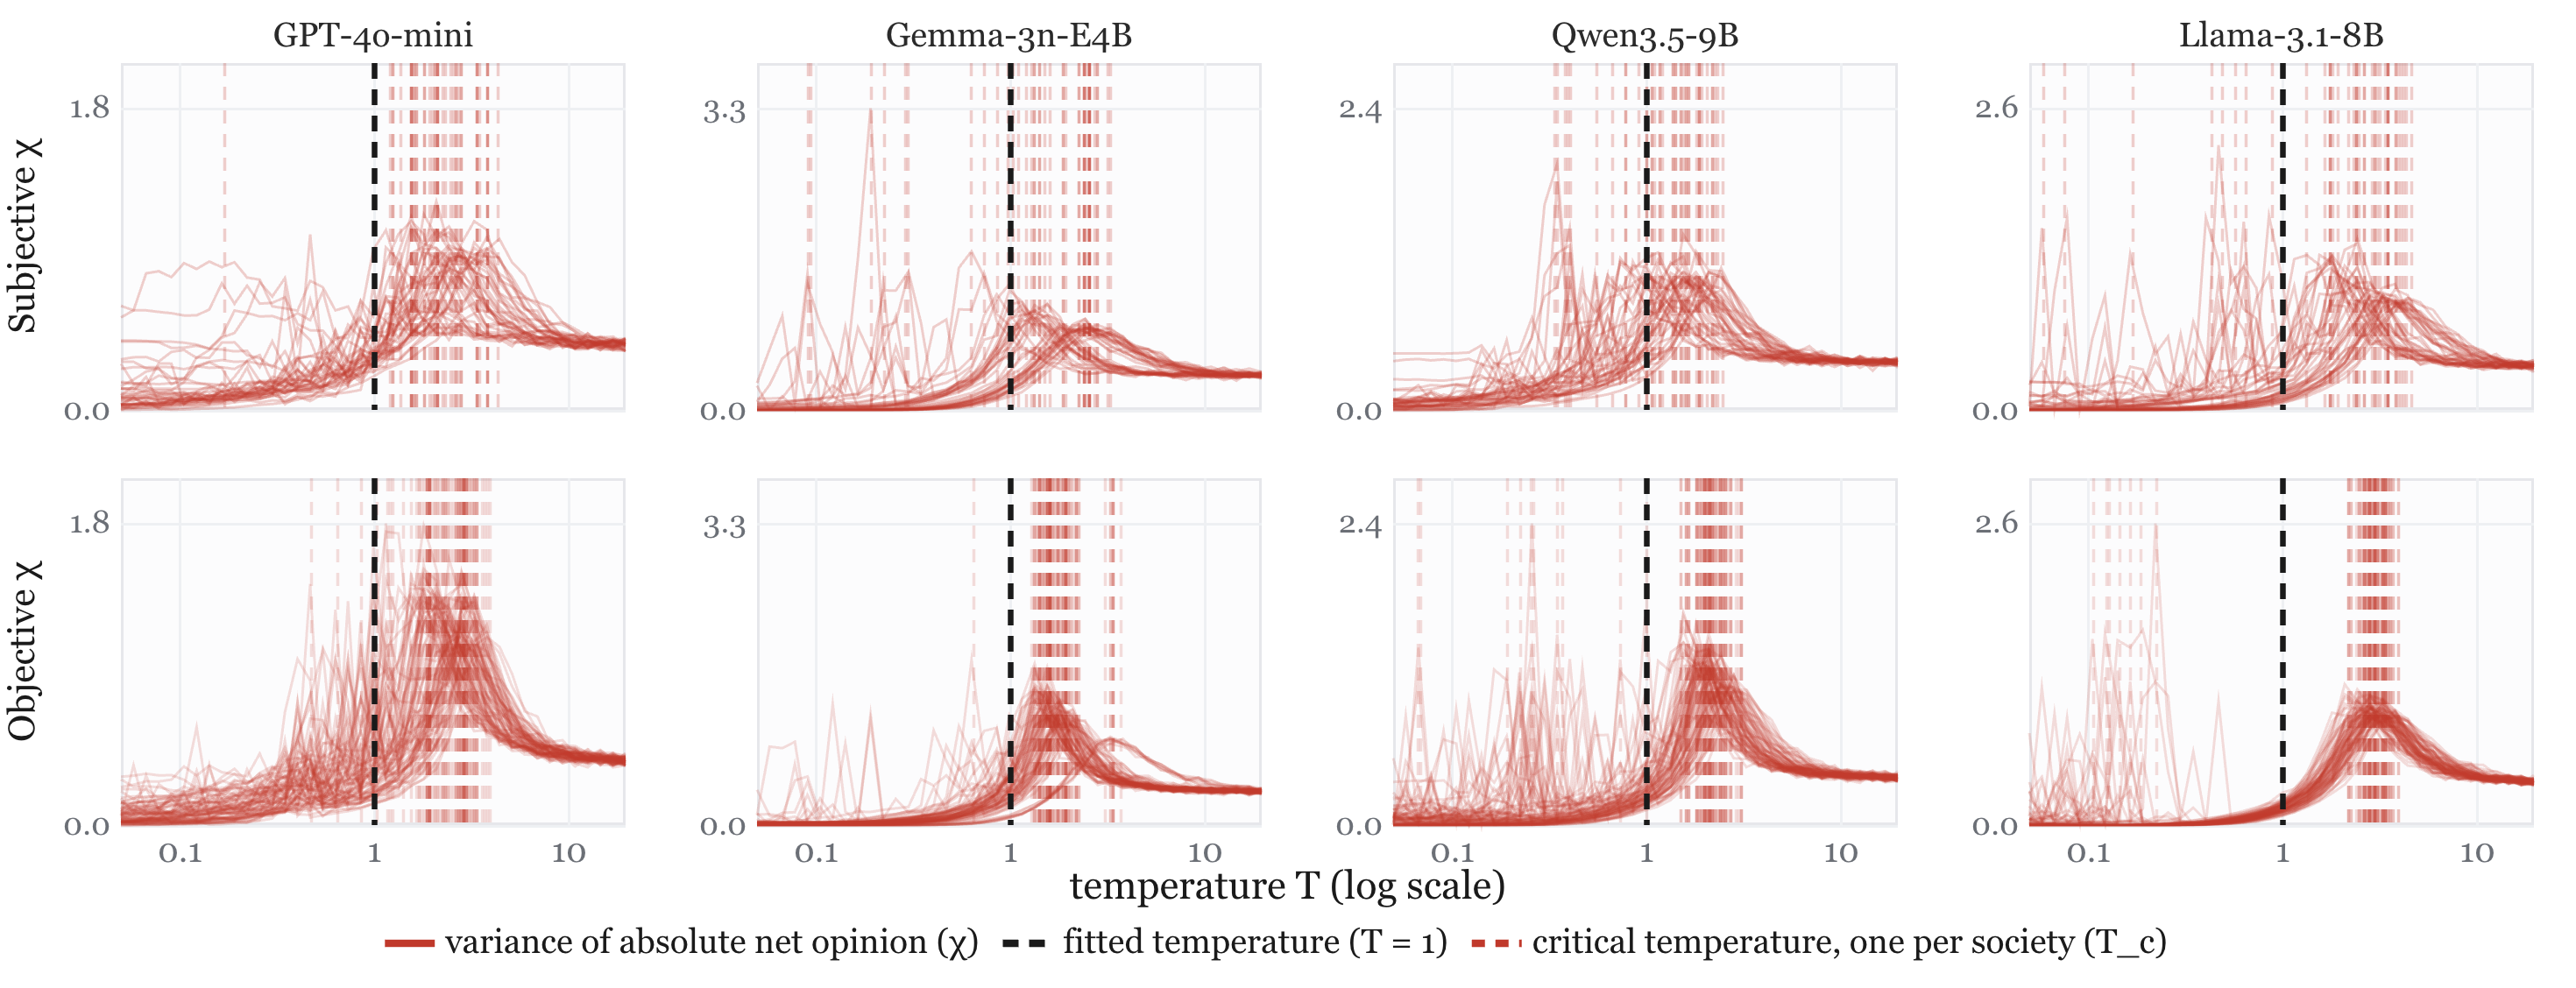
\includegraphics[width=0.99\textwidth]{main/Figures/apx_08_temperature_sweep_grid.png}
\caption{\textit{Figure~\ref{fig:agent_model_tc_mean_test_J03_fitted_nomf_tcmean} with each question-$J$ pair presented individually.} Figure~\ref{fig:agent_model_tc_mean_test_J03_fitted_nomf_tcmean} in
Section~\ref{sec:results_temperature} reports the across-community mean of these curves and the
across-community mean of their $\chi$-peak $\mathcal{T}_c$'s. This figure shows the same sweep without any
averaging with one curve and one $\mathcal{T}_c$ line per group. \label{fig:agent_model_tc_mean_test_J03_fitted_nomf_tcmean_qea}}
\end{figure}





This appendix explains how the critical temperatures in Section~\ref{sec:results_temperature} are computed. To avoid confusion, we begin by clarifying that this experiment does not modify the language model’s temperature. Instead, it modifies the temperature of the fitted model, as described below.

\textit{Setup.} The experiment covers every question in the test set and four in-distribution random graphs. Four graphs $\times$ the test question bank gives $80$
objective and $40$ subjective groups per model, each with four independent episodes. 

\textit{Model.} The sweep uses the parameters of the three-coupling discrete update rule.

\textit{Introducing Temperature.} Our fitted rule is
$P\big(s_i(t{+}1)=+1\big) = \sigma\big(h_i\big)$. Reintroducing the temperature divides that
logit by $\mathcal{T}$,
\[
P\big(s_i = +1\big) \;=\; \sigma\!\left(\frac{h_i}{\mathcal{T}}\right),
\]
so the $\mathcal{T}=1$ point of the sweep is the fitted model itself.

\textit{Initialization.} We call a $J$ paired with a question a \textit{group}. For each group, we have taken $4$ independent trajectories in our experiments. The $4$ trajectories are considered as the different rollouts of the same system in the temperature sweep as well. We initialize a group at each of the four starting points at $t=0$ from the $4$ independently sampled trajectories.  

\textit{Procedure.} We sweep $41$ log-spaced temperatures from $0.05$ to $20$.\footnote{$0.050, 0.058, 0.067, 0.078, 0.091, 0.106, 0.123, 0.143, 0.166, 0.193, 0.224, 0.260, 0.302, 0.350, 0.407, 0.473, 0.549, 0.638, 0.741, 0.861, 1.000,\\ 1.162, 1.349, 1.567, 1.821, 2.115, 2.456, 2.853, 3.314, 3.850, 4.472, 5.195, 6.034, 7.009, 8.142, 9.457, 10.986, 12.761, 14.823, 17.218, 20.000
$} At each
temperature, we run the model for $500$ synchronous steps. We discard the first $200$ (to account for the time it takes for the community to reach equilibrium) and retain the last $300$. During this run, each agent's opinion in the next step $s_i = \pm1$ is sampled with probability $\sigma(h_i/\mathcal{T})$.

\textit{Observables.} From the $300$ steps of the group trajectories, we compute $\chi \;=\; N\,\mathrm{Var}_t\big(|n(t)|\big)$. The four independent trajectories per group are used as four independent initial conditions that are then averaged into one $\chi$ curve per group.

\textit{Locating $\mathcal{T}_c$.} A group's $\mathcal{T}_c$ is the location of its $\chi$ peak. Since the grid is
coarse relative to the width of the peak, we fit a parabola through the maximizing
grid point and its two neighbors in $\log \mathcal{T}$ and take the vertex, which resolves $\mathcal{T}_c$ below the
spacing of the $41$-point grid.

\subsection{Predictability of Group Archetypes}\label{apdx:replica_predictability}

\begin{figure}[h]
    \centering
    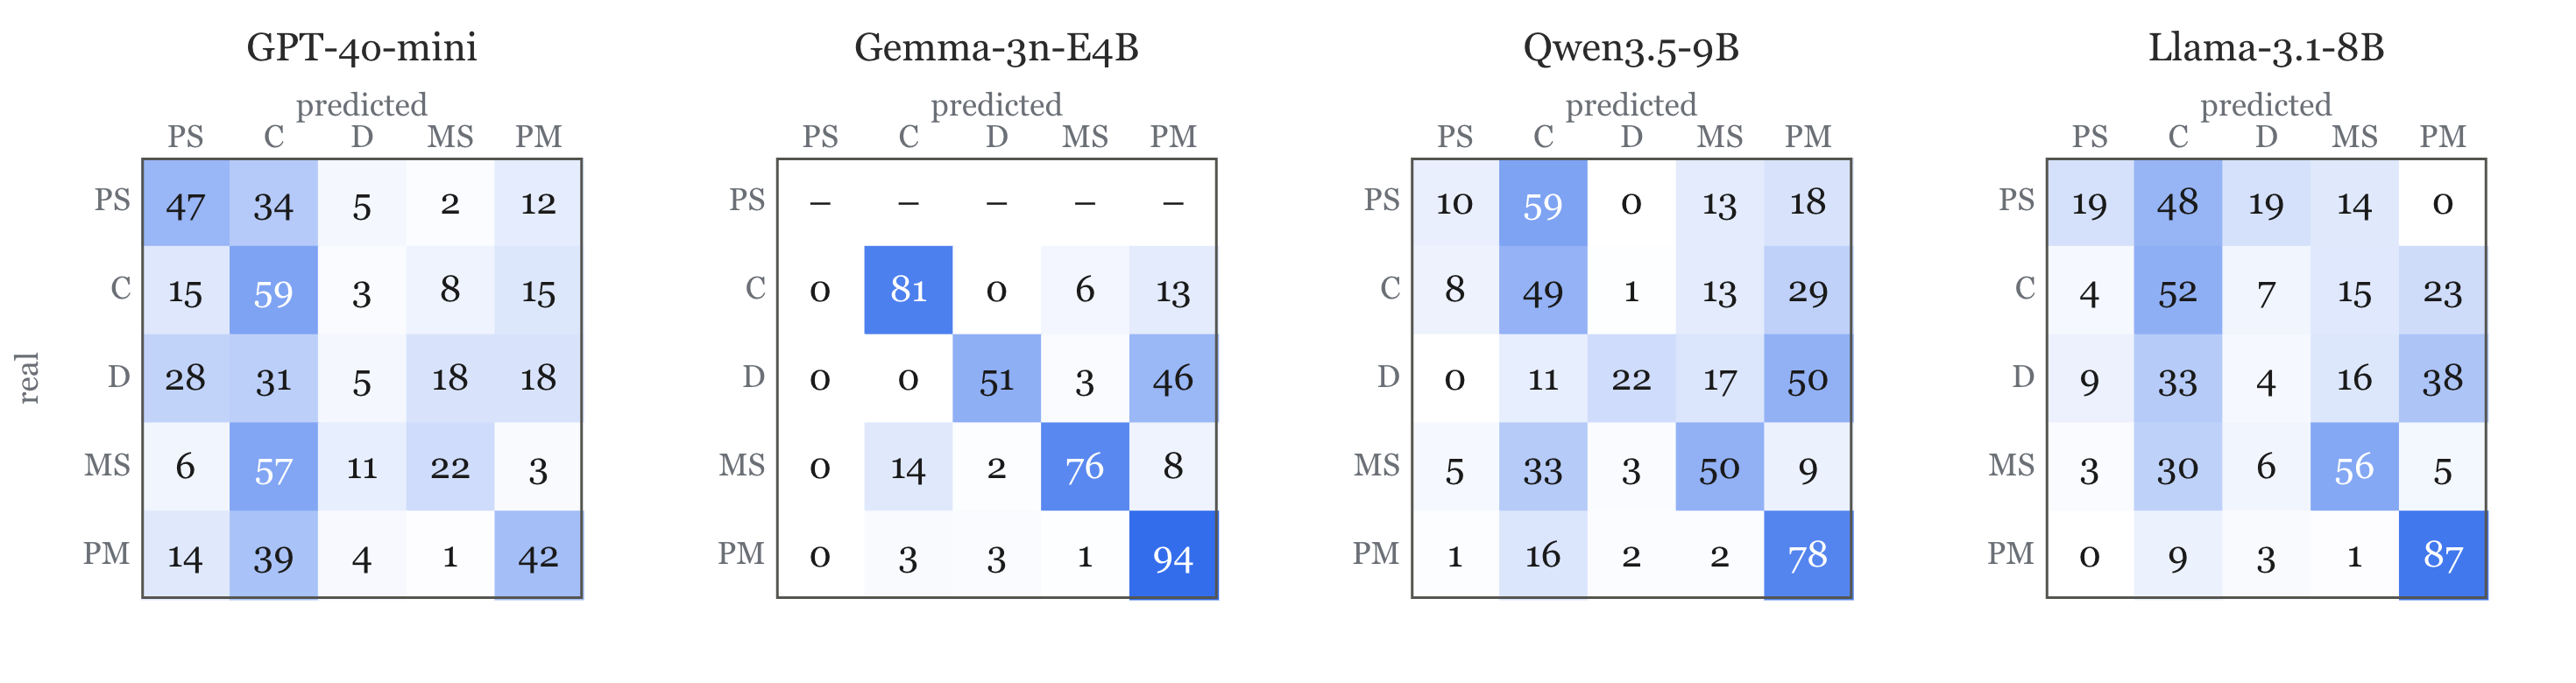
\includegraphics[width=0.99\textwidth]{main/Figures/apx_09_replica_predictability_objective.png}
    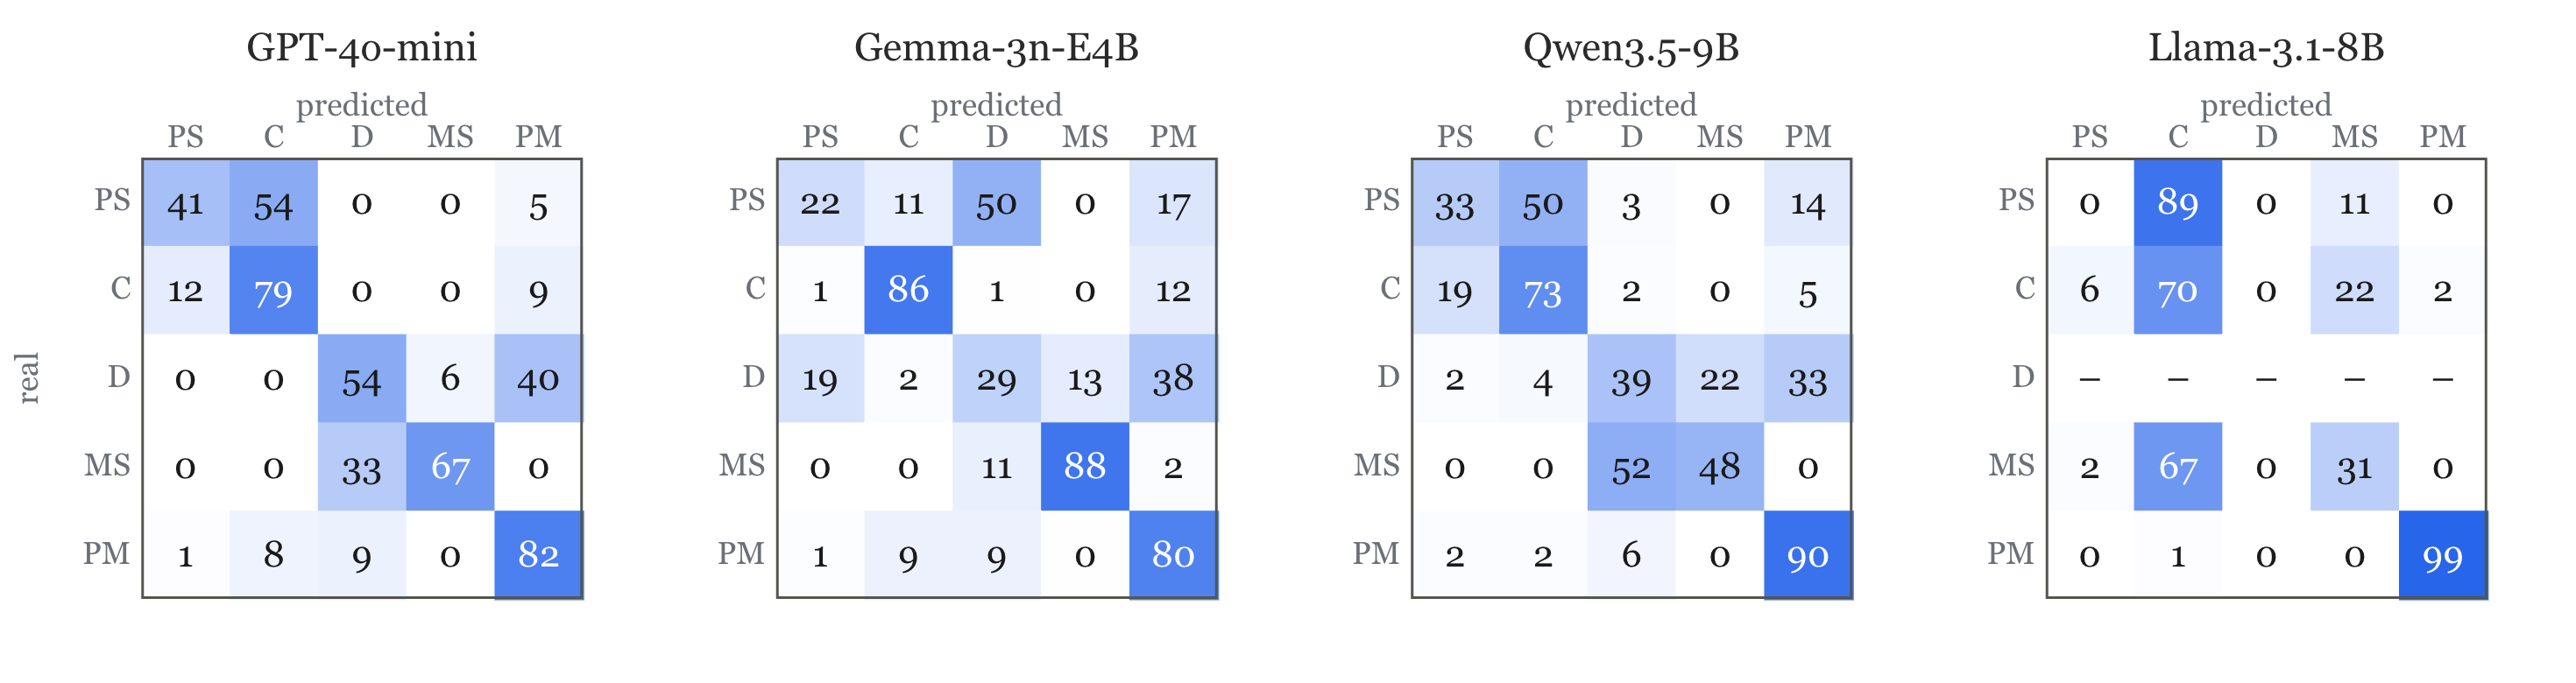
\includegraphics[width=0.99\textwidth]{main/Figures/apx_10_replica_predictability_subjective.png}
\caption{\textit{Predictability of the Group Archetypes (row 1: objective; row 2: subjective).} For every (question $\times$ graph) pair, we assess agreement among the $4$ independently sampled episodes. For this analysis, we use test questions and $4$ random graphs as our $J$s. For each question--$J$ pair, we use the group archetype of one of the $4$ trajectories as the predicted group archetype. We then use the remaining $3$ group trajectories as the test set to construct a confusion matrix for predicting the correct group archetype. We repeat this process, using each of the $4$ trajectories in turn as the prediction and the remaining $3$ as the test set, in a cross-validation manner, and report the \textit{``cross-validated''} confusion matrix. Because every trajectory takes its turn as the predictor, the cross-validated matrix is symmetric in raw counts. Row normalization makes the confusion matrix asymmetric. A row of the confusion matrix shows how often, for example, a \textit{persistent split} trajectory is predicted as each of the other group archetypes. If the repeated samples always matched, we would observe a diagonal confusion matrix with $100$ on the diagonal. \label{fig:predictability_macro_subjective_test_J03_cv_row}}\end{figure}

\newpage
\subsection{Flow of Opinion} 
\label{apdx:f1}


\begin{figure}[h]
    \centering
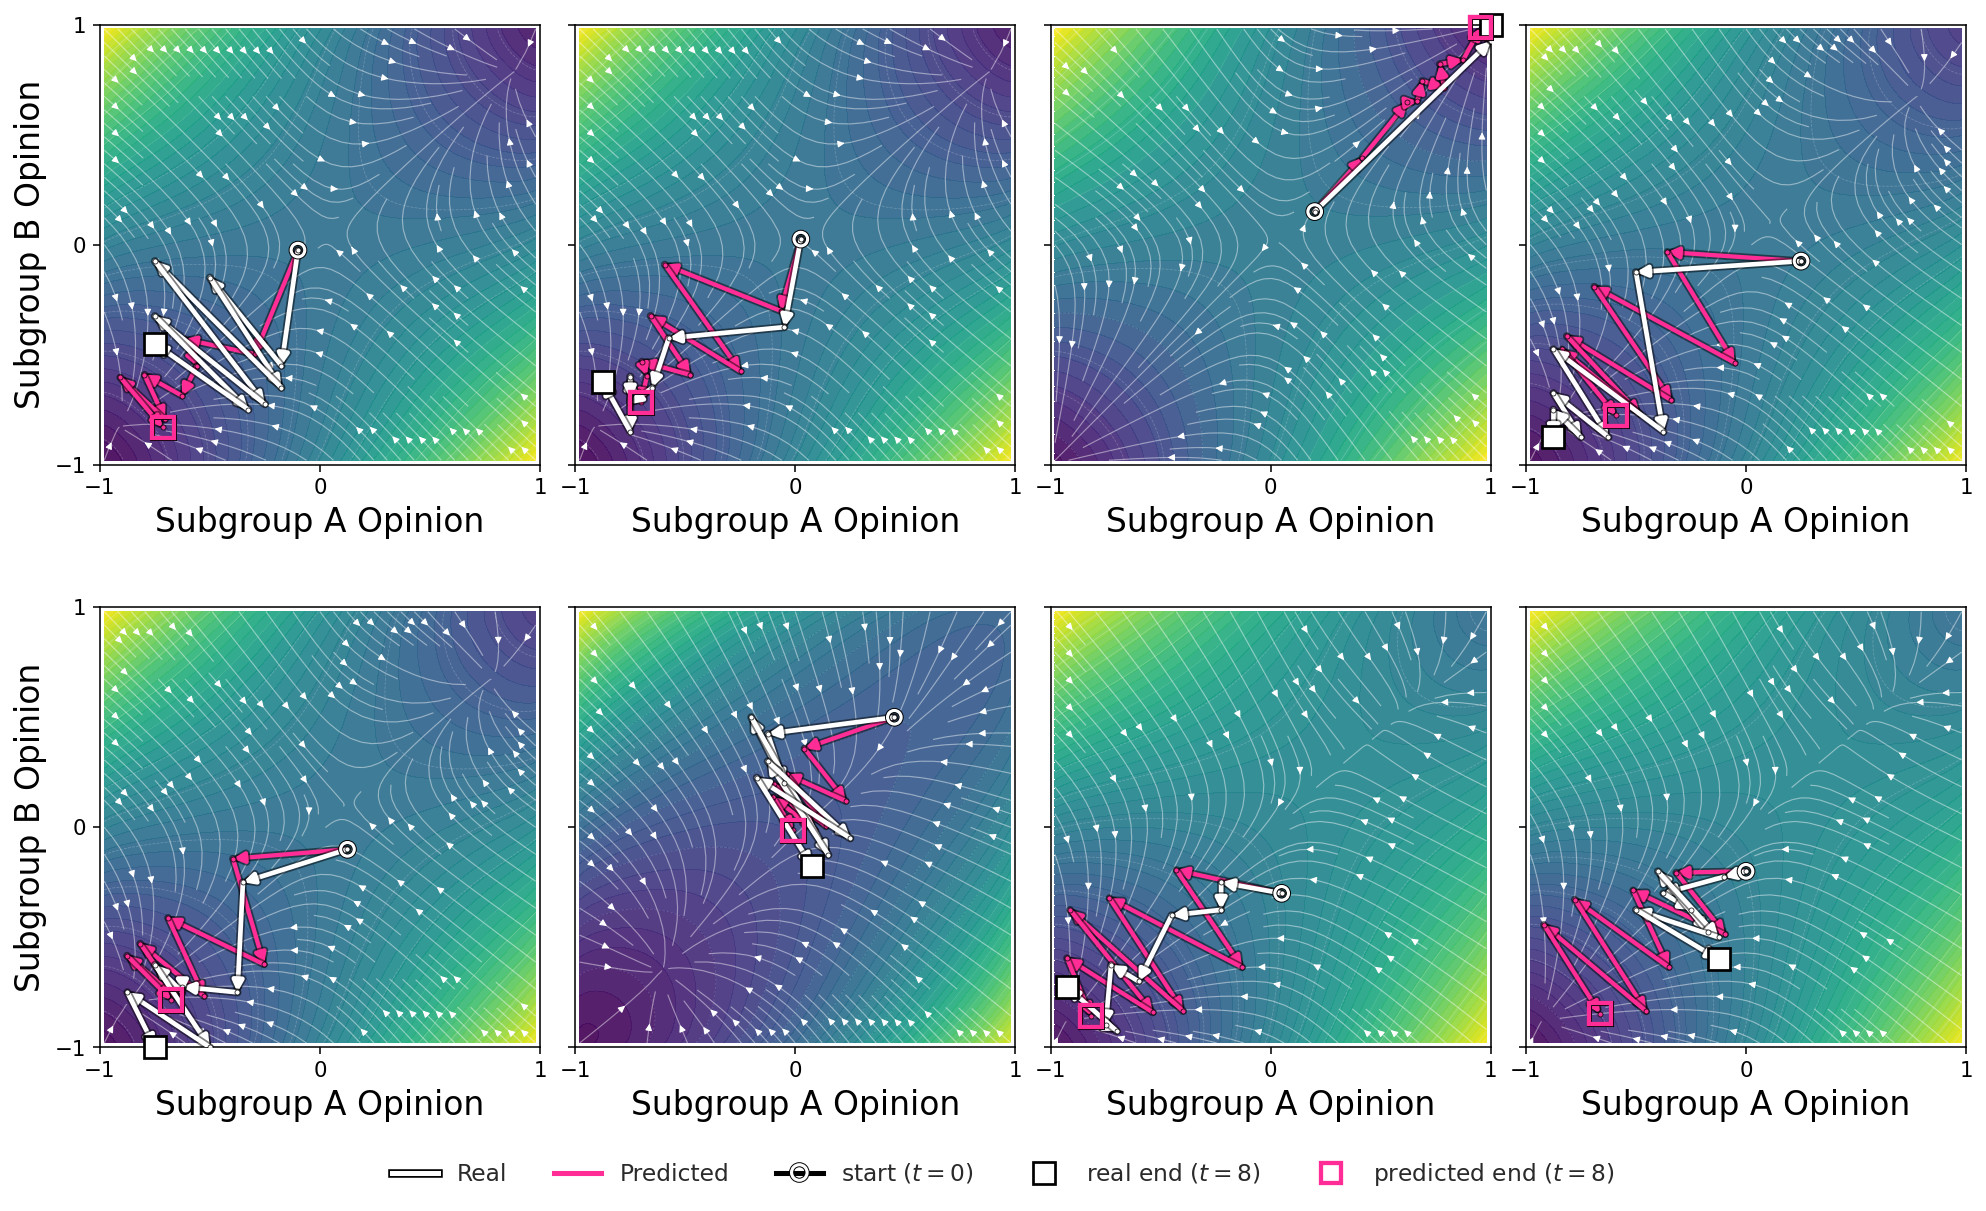
\includegraphics[width=0.99\textwidth]{main/Figures/apx_11_opinion_flow_examples.png}
\caption{\textit{Flow of opinion predicted by the continuous three coupling model.} Each panel is one
group of 32 language-model agents interacting about a question over eight rounds. The axes are the average opinions of the two subgroups. The background shows our fitted model's predictions, with energy represented by colors and the predicted flow (at the continuous time limit) represented by streamlines in the background. White indicates the observed transitions, while pink shows the model's predicted rollout from the initial opinions at $t=0$, that updates the agents synchronously at discrete time intervals $t=1,\dots, T$.  
}
\end{figure}
\begin{figure}[h!]
    \centering
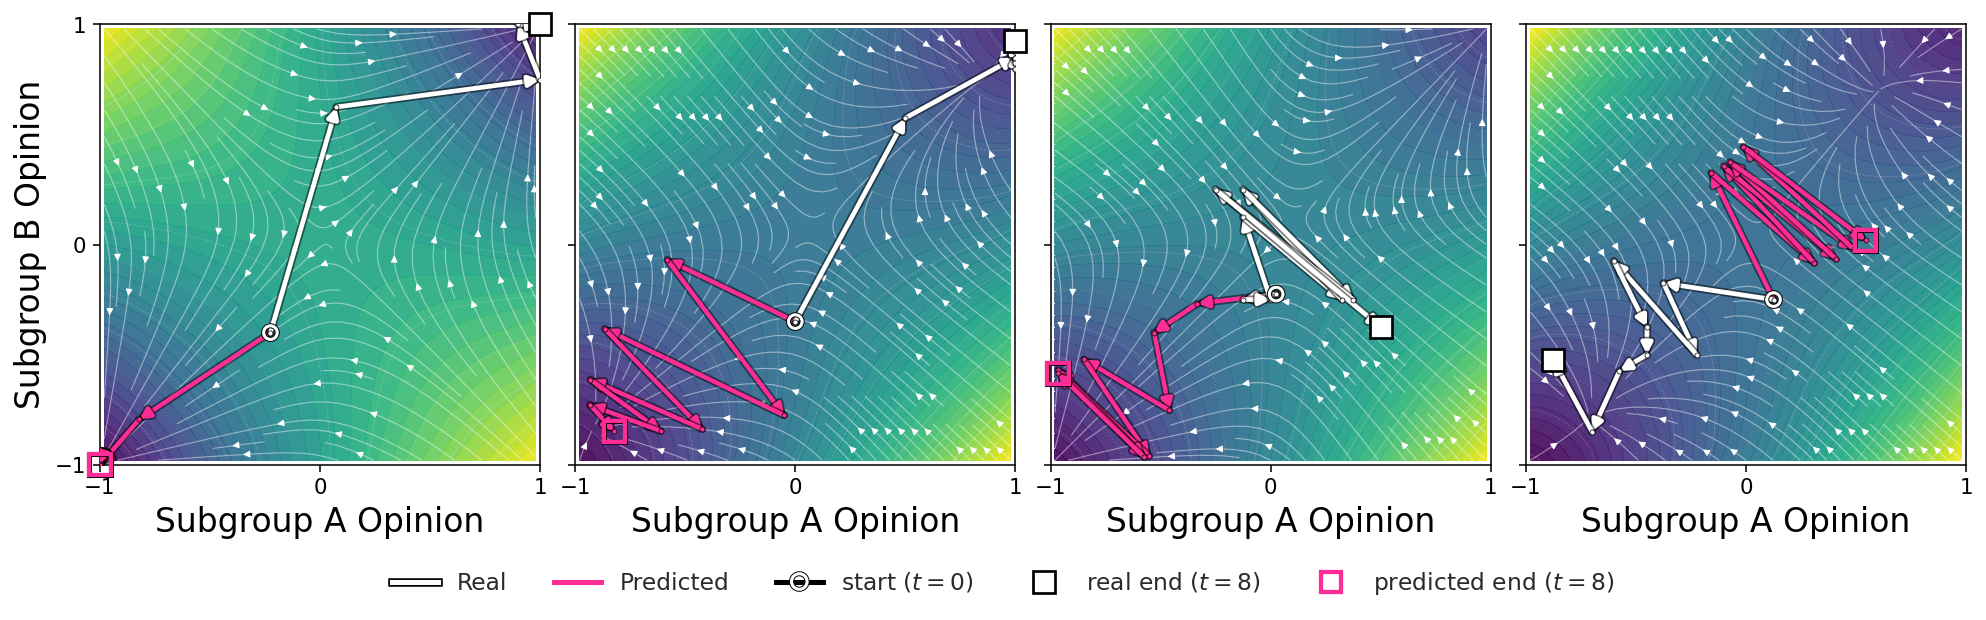
\includegraphics[width=0.99\textwidth]{main/Figures/apx_12_opinion_flow_mismatches.png}
\caption{\textit{Four example group trajectories where predictions do not match the observations.}
}
\end{figure}
\textit{Splitting into groups.} We split the agents into two subgroups based on their opinion at $t=0$. The $N=32$ agents are ranked by their round-0 opinion $\bar{o}_i(0)$; the top half forms group $A$ and the bottom half group $B$, so the two
subgroups always have equal size ($16$ and $16$) and $A$ is by construction the side that starts higher, $n_A(0)\ge n_B(0)$, where $n_A(0)$ denotes the net opinion of the agents in subgroup A. Ties are broken by the following round, then the one after.

At each point on a $220\times220$ grid, we record the net opinions of agents in $A$, $n_A(t)$, and agents in $B$, $n_B(t)$. We generate rollouts and plot the subgroup net opinions at each timestep. The white path shows the real community’s per-round net opinions in the same two-dimensional space, while the pink path shows a rollout from the fitted continuous three-coupling update rule, initialized from the same state. We show selected rollouts on the held-out test set of questions.


\stopcontents[apx]
\newpage
